\chapter{Primer encuentro con anillos\texorpdfstring{\\}{ }de números}

En este capítulo introductorio vamos a definir los campos y anillos de números y
para motivar su estudio, veremos varios ejemplos de sus aplicaciones a los
problemas de la teoría de números clásica.

%%%%%%%%%%%%%%%%%%%%%%%%%%%%%%%%%%%%%%%%%%%%%%%%%%%%%%%%%%%%%%%%%%%%%%%%%%%%%%%%

% \pdfbookmark{Clase 1 (10/08/20)}{clase-1}
\section{Campos de números}
\marginpar{\small Clase 1 \\ 10/08/20}

Como sugiere el nombre del curso, nuestro objeto de estudio son los
\textbf{números algebraicos} que son elementos de $\overline{\QQ}$, la cerradura
algebraica del campo de números racionales $\QQ$.

\begin{definicion}
  Un número $\alpha \in \CC$ es \textbf{algebraico} si este satisface alguna
  relación algebraica
  $$a_n \alpha^n + a_{n-1} \alpha^{n-1} + \cdots + a_1 \alpha + a_0 = 0,$$
  donde $a_0,a_1,\ldots,a_n \in \QQ$ y $a_n \ne 0$.
\end{definicion}

Por supuesto, siempre se pueden normalizar los coeficientes para obtener un
polinomio mónico con $a_n = 1$. Si además se puede escoger un polinomio mónico
con \emph{coeficientes enteros}, se dice que $\alpha$ es un
\textbf{entero algebraico}.

\begin{definicion}
  Se dice que $\alpha \in \CC$ es un \term{entero algebraico} si
  $$\alpha^n + a_{n-1} \alpha^{n-1} + \cdots + a_1 \alpha + a_0 = 0,$$
  para algunos $a_0,a_1,\ldots,a_{n-1} \in \ZZ$.
\end{definicion}

\begin{ejemplo}
  El número $\alpha = \frac{1 + \sqrt{5}}{2}$ es un entero algebraico, ya que
  cumple la relación
  \[ \alpha^2 - \alpha - 1 = 0. \qedhere \]
\end{ejemplo}

Todos los enteros algebraicos forman un subanillo de $\overline{\QQ}$
(no es algo inmediato; lo veremos más adelante en el curso).

\vspace{1em}

Los números algebraicos viven en campos de números.

\begin{definicion}
  Un \textbf{campo de números} es una extensión finita $K/\QQ$.
\end{definicion}

Recordemos que por una extensión \textbf{finita} se entiende una extensión de
grado $[K : \QQ] = \dim_\QQ K$ finito.

\begin{ejemplo}
  Sea $d$ un entero \textbf{libre de cuadrados}\footnote{Es decir,
    tal que $n^2 \nmid d$ para ningún $n > 1$} (posiblemente negativo). Entonces,
  $$\QQ \subset \QQ (\sqrt{d}) = \{ a + b\sqrt{d} \mid a,b \in \QQ \}$$
  es una extensión de $\QQ$ de grado $2$. A saber, como una base sobre $\QQ$ se
  puede tomar $\{ 1, \sqrt{d} \}$.
\end{ejemplo}

\begin{ejemplo}
  Sea $f \in \QQ [x]$ un polinomio irreducible. En este caso el anillo cociente
  $\QQ [x]/(f)$ es un campo y es una extensión de $\QQ$ de grado $\deg f$.
  Si $\alpha$ es una raíz de $f$, entonces el homomorfismo de evaluación
  $$\QQ [x] \to \CC, \quad g \mapsto g(\alpha)$$
  induce un isomorfismo
  $$\QQ (\alpha) \cong \QQ [x]/(f).$$
  Notamos que el objeto a la derecha es puramente algebraico.

  De hecho, toda extensión finita de $\QQ$ es isomorfa a una de la forma
  $\QQ (\alpha) \cong \QQ [x]/(f)$; este es el contenido del
  \textbf{teorema del elemento primitivo} (véanse los ejercicios).
\end{ejemplo}

\begin{ejemplo}
  Sea $\zeta_n = \exp (2\pi i/n)$ una raíz $n$-ésima primitiva. El polinomio
  mínimo de $\zeta_n$ es el \textbf{$n$-ésimo polinomio ciclotómico}
  \[ \Phi_n = \prod_{\substack{1 \le k < n \\ \gcd (k,n) = 1}} (x - \zeta_n^k)
       \in \ZZ [x]. \]

  El hecho de que el polinomio de arriba tiene coeficientes enteros y es
  irreducible no es tan inmediato. El lector que no conoce los polinomios
  ciclotómicos puede revisar el Apéndice~\ref{ap:polinomios-ciclotomicos}.

  El \textbf{$n$-ésimo campo ciclotómico}
  $$\QQ (\zeta_n) \cong \QQ [x] / (\Phi_n)$$
  es una extensión de grado $\phi (n)$ de $\QQ$.

  Se tiene $\QQ (\zeta_m) = \QQ (\zeta_n)$ para $m < n$ si y solamente si $m$ es
  impar y $n = 2m$. Esto también se refleja en la identidad para los polinomios
  ciclotómicos $\Phi_{2m} (x) = \Phi_m (x)$.
\end{ejemplo}

%%%%%%%%%%%%%%%%%%%%%%%%%%%%%%%%%%%%%%%%%%%%%%%%%%%%%%%%%%%%%%%%%%%%%%%%%%%%%%%%

\section{Anillos de números}

La siguiente terminología es un poco menos común, pero será útil en nuestro
curso.

\begin{definicion}
  Un \textbf{anillo de números} es un subanillo de un campo de números.
\end{definicion}

\begin{ejemplo}
  Los anillos $\ZZ$,
  \begin{align*}
    \ZZ \Bigl[\frac{1}{n}\Bigr] & =
        \Bigl\{ \frac{a}{n^k} \Bigm| a \in \ZZ, \, k = 0,1,2,\ldots \Bigr\},\\
    \ZZ_{(p)} & = \Bigl\{ \frac{a}{b} \Bigm| p \nmid b \Bigr\}
  \end{align*}
  (para $n > 0$ y $p$ primo fijos) son anillos de números, siendo subanillos de
  $\QQ$. Los anillos $\ZZ \Bigl[\frac{1}{n}\Bigr]$ y $\ZZ_{(p)}$ son diferentes
  \textbf{localizaciones} de $\ZZ$.
\end{ejemplo}

\begin{ejemplo}
  Si $d$ es un entero libre de cuadrados, entonces
  $$\ZZ [\sqrt{d}] = \{ a + b\sqrt{d} \mid a,b\in \ZZ \}$$
  es un anillo de números, siendo un subanillo de $\QQ (\sqrt{d})$. Este es un
  $\ZZ$-módulo libre de rango $2$.

  Si $d \equiv 1 \pmod{4}$, se puede considerar el anillo más grande
  \[ \ZZ \Bigl[\frac{1 + \sqrt{d}}{2}\Bigr] =
         \Bigl\{ a + b\,\frac{1 + \sqrt{d}}{2} \Bigm| a,b \in \QQ \Bigr\}
             \subset \QQ (\sqrt{d}). \]
  Notamos que el número $\alpha = \frac{1 + \sqrt{d}}{2}$ es un entero
  algebraico, ya que este satisface la relación
  $$\alpha^2 - \alpha - \frac{d-1}{4} = 0.$$
  De nuevo, $\ZZ \Bigl[\frac{1 + \sqrt{d}}{2}\Bigr]$ es un $\ZZ$-módulo libre de
  rango $2$.
\end{ejemplo}

\begin{ejemplo}
  El anillo
  $$\ZZ [\zeta_n] = \Bigl\{ \sum_k a_k \, \zeta_n^k \mid a_k \in \ZZ \Bigr\}$$
  es un anillo de números, siendo un subanillo del campo ciclotómico
  $\QQ (\zeta_n)$.
\end{ejemplo}

Una clase importante de anillos de números son órdenes.

\begin{definicion}
  Un anillo de números $R \subset K$ que es finitamente generado como
  $\ZZ$-módulo se llama un \textbf{orden} en su campo de fracciones
  $\Frac R \subseteq K$.
\end{definicion}

Puesto que un campo de números $K$ como un grupo aditivo no tiene elementos
de torsión, notamos que un orden es un $\ZZ$-módulo \emph{libre}.

\begin{ejemplo}
  Los anillos de números $\ZZ [\sqrt{d}]$ y $\ZZ [\zeta_n]$ son órdenes.
  En general, si $f \in \ZZ [x]$ es un polinomio mónico irreducible, entonces
  $\ZZ [x]/(f)$ es un orden de rango $\deg f$. Este anillo es isomorfo a
  $\ZZ [\alpha]$ donde $\alpha$ es una raíz de $f$. Notamos que $\ZZ [x]/(f)$
  naturalmente se identifica con un subanillo de $\QQ [x]/(f)$:
  $$\ZZ [\alpha] \subset \QQ (\alpha).$$
  Este es el candidato más obvio para un subanillo en un campo de números.
  Sin embargo, más adelante veremos que no es siempre la mejor opción.

  Notamos que en este ejemplo $f$ es un polinomio mónico con coeficientes
  enteros, así que $\alpha$ es un entero algebraico. En el caso contrario,
  si $\alpha$ no es un entero algebraico, $\ZZ [\alpha]$ no será finitamente
  generado como un $\ZZ$-módulo.
\end{ejemplo}

\begin{ejemplo}
  Por otra parte, los anillos como $\QQ$, $\ZZ \Bigl[\frac{1}{n}\Bigr]$ y
  $\ZZ_{(p)}$ no son órdenes (ejercicio).
\end{ejemplo}

%%%%%%%%%%%%%%%%%%%%%%%%%%%%%%%%%%%%%%%%%%%%%%%%%%%%%%%%%%%%%%%%%%%%%%%%%%%%%%%%

\section{Primeros cálculos en PARI/GP}

Durante el curso trataremos de ver ejemplos de cálculos en el programa
PARI/GP. Para descargarlo y consultar la documentación, consulte la página
\begin{center}
  \url{https://pari.math.u-bordeaux.fr/}
\end{center}
También recomiendo el libro \cite{Rodriguez-Villegas-2007} enfocado en la
exploración de la teoría de números a través de cálculos en PARI/GP.

\vspace{1em}

Ya que estábamos hablando de números algebraicos, la función
\texttt{algdep($x$,$d$)} busca una relación algebraica para $x$ de grado
$\le d$. Por ejemplo,
\begin{shaded}
\begin{verbatim}
? algdep((sqrt(13)+1)/2, 2)
% = x^2 - x - 3
? algdep(fibonacci(101)/fibonacci(100)*1.0, 2)
% = x^2 - x - 1
? algdep (exp (2*Pi*I/7), 6)
% = x^6 + x^5 + x^4 + x^3 + x^2 + x + 1
? algdep (sqrt(2) + sqrt(3), 4)
% = x^4 - 10*x^2 + 1
? algdep (Pi,5)
% = 37542*x^5 - 69665*x^4 - 134081*x^3 - 77323*x^2 + 40979*x + 89174
? subst(%,x,Pi)
% = -1.7092371337382136939 E-26
\end{verbatim}
(El número $\pi$ es trascendente, así que no hay que esperar una relación
algebraica razonable.)
\end{shaded}

Dado que todos los campos de números son de la forma $\QQ [x]/(f)$ para
un polinomio irreducible $f$, para hacer cálculos en ellos basta saber trabajar
con los polinomios módulo $f$. Esto se hace mediante la división con resto, pero
en práctica se puede usar PARI/GP. Allí la expresión \texttt{Mod($g$,$f$)} denota
el polinomio $g$ módulo $f$. Si queremos olvidar de que $g$ se considera módulo
$f$, se puede usar la función \texttt{lift($x$)}

Por ejemplo, para calcular las potencias de $1 + \sqrt{2}$, podemos hacer
lo siguiente:
\begin{shaded}
\begin{verbatim}
? u = Mod (1+x, x^2-2);
? vector (10,i,u^i)
% = [Mod(x + 1, x^2 - 2), Mod(2*x + 3, x^2 - 2), Mod(5*x + 7, x^2 - 2),
     Mod(12*x + 17, x^2 - 2), Mod(29*x + 41, x^2 - 2),
     Mod(70*x + 99, x^2 - 2), Mod(169*x + 239, x^2 - 2),
     Mod(408*x + 577, x^2 - 2), Mod(985*x + 1393, x^2 - 2),
     Mod(2378*x + 3363, x^2 - 2)]
? lift (%)
% = [x + 1, 2*x + 3, 5*x + 7, 12*x + 17, 29*x + 41, 70*x + 99,
     169*x + 239, 408*x + 577, 985*x + 1393, 2378*x + 3363]
\end{verbatim}
\end{shaded}

Para verificar si un polinomio es irreducible, se puede usar
\texttt{polisirreducible($f$)}, mientras que \texttt{factor($f$)} encuentra los
factores irreducibles.
\begin{shaded}
\begin{verbatim}
? f = polcyclo(12)
% = x^4 - x^2 + 1

? polisirreducible(f)
% = 1
? factor (f*Mod(1,2))
% = 
[Mod(1, 2)*x^2 + Mod(1, 2)*x + Mod(1, 2) 2]

? factor (f*Mod(1,3))
% = 
[Mod(1, 3)*x^2 + Mod(1, 3) 2]

? factor (f*Mod(1,5))
% = 
[Mod(1, 5)*x^2 + Mod(2, 5)*x + Mod(4, 5) 1]
[Mod(1, 5)*x^2 + Mod(3, 5)*x + Mod(4, 5) 1]

? factor (x^6-1)
% = 
[      x - 1 1]
[      x + 1 1]
[x^2 - x + 1 1]
[x^2 + x + 1 1]
\end{verbatim}
\end{shaded}

El polinomio mínimo y el polinomio característico se encuentran mediante
\texttt{minpoly($x$)} y \texttt{charpoly($x$)} respectivamente:
\begin{shaded}
\begin{verbatim}
? charpoly (Mod (x + x^-1, polcyclo (5)))
% = x^4 + 2*x^3 - x^2 - 2*x + 1
? factor(%)
% = 
[x^2 + x - 1 2]

? minpoly (Mod (x + x^-1, polcyclo (5)))
% = x^2 + x - 1
\end{verbatim}
\end{shaded}

%%%%%%%%%%%%%%%%%%%%%%%%%%%%%%%%%%%%%%%%%%%%%%%%%%%%%%%%%%%%%%%%%%%%%%%%%%%%%%%%

\section{Reciprocidad cuadrática mediante sumas de Gauss en \texorpdfstring{$\ZZ [\zeta_p]$}{ℤ[ζₚ]}}
\label{sec:reciprocidad-cuadratica}

\marginpar{\small Lectura\\adicional}

Existen muchísimas pruebas de la ley de reciprocidad cuadrática, y en esta
seccón vamos a ver la prueba de Gauss basada en cálculos ingeniosos en el anillo
ciclotómoco $\ZZ [\zeta_p]$. Este es un ejemplo curioso de cómo propiedades
de los números enteros $\ZZ$ se establecen al pasar a un anillo más grande.

\begin{definicion}
  Sea $p$ un número primo fijo. Para un número entero $a$ tal que $p\nmid a$
  el \term{símbolo de Legendre} se define mediante
  \[ \legendre{a}{p} = \begin{cases}
    +1, & a\text{ es un cuadrado módulo }p,\\
    -1, & a\text{ no es un cuadrado módulo }p.
  \end{cases} \]
  Además, para $p \mid a$ se pone $\legendre{a}{p} = 0$.
\end{definicion}

De la definición está claro que si $a \equiv b \pmod{p}$, entonces
$\legendre{a}{p} = \legendre{b}{p}$. Recordemos que el grupo multiplicativo
$\FF_p^\times$ es cíclico
(véase \ref{cor:grupo-multiplicativo-de-campo-finito}), lo que significa que
existe un generador $x\in \FF_p^\times$ tal que
$$\FF_p^\times = \{ 1, x, x^2, x^3, \ldots, x^{p-2} \}.$$
Entonces, $x^k$ es un cuadrado si y solamente si $k$ es par.
De aquí se ve fácilmente que el símbolo de Legendre es multiplicativo:
$$\legendre{ab}{p} = \legendre{a}{p}\,\legendre{b}{p}.$$
Entonces, se trata de un homomorfismo
$$\legendre{\cdot}{p}\colon \FF_p^\times \to \{ \pm 1 \}.$$

Para calcular el símbolo de Legendre, se usa el siguiente resultado, descubierto
por Gauss.

\begin{teorema}[Reciprocidad cuadrática]
  Sean $p$ y $q$ diferentes primos impares. Entonces,
  \[ \legendre{q}{p} =
     (-1)^{\frac{p-1}{2}\,\frac{q-1}{2}}\,\legendre{p}{q}.\]
  Además, se cumple
  \begin{align*}
    \legendre{-1}{p} & = (-1)^{\frac{p-1}{2}},\\
    \legendre{2}{p} & = (-1)^{\frac{p^2-1}{8}}.
  \end{align*}
\end{teorema}

\begin{ejemplo}
  \label{ejemplo:legendre--3}
  Para $p \ne 3$ calculemos el símbolo de Legendre $\legendre{-3}{p}$.
  Tenemos
  \[ \legendre{-3}{p} = \legendre{-1}{p}\,\legendre{3}{p} =
       (-1)^{\frac{p-1}{2}}\,(-1)^{\frac{3-1}{2}\,\frac{p-1}{2}}\,\legendre{p}{3} =
         \legendre{p}{3}. \]
  El único cuadrado no nulo módulo $3$ es $1$, así que
  \[ \legendre{-3}{p} = \begin{cases}
    +1, & \text{si } p\equiv 1 \pmod{3},\\
    -1, & \text{si } p\equiv 2 \pmod{3}.
  \end{cases} \]
  Por ejemplo,
  \[ -3 \equiv 2^2 ~ (7), -3 \equiv 6^2 ~ (13), -3 \equiv 4^2 ~ (19), -3 \equiv 11^2 ~ (31), -3 \equiv 16^2 ~ (37). \qedhere \]
\end{ejemplo}

\subsection{Congruencia de Euler y leyes suplementarias}

Primero, nos servirá la siguiente interpretación del símbolo de Legendre.

\begin{lema}[Congruencia Euler]
  Para $p \ne 2$ y $a$ tal que $p \nmid a$ se tiene
  $$\legendre{a}{p} \equiv a^{\frac{p-1}{2}} \pmod{p}.$$

  \begin{proof}
    Sea $x$ un generador de $\FF_p^\times$. Tenemos $[a]_p = x^i$ para algún
    $i$, y este es un cuadrado en $\FF_p^\times$ si y solamente si $i$ es
    par. Luego,
    $$[a]_p^{\frac{p-1}{2}} = x^{i\frac{p-1}{2}}.$$
    Si $i$ es par, entonces $i\frac{p-1}{2}$ es divisible por
    $p-1 = \#\FF_p^\times$, así que
    $$x^{i\frac{p-1}{2}} = 1$$
    (usando que $|\FF_p^\times| = p-1$). Si $i$ es impar, entonces
    $i\frac{p-1}{2}$ no es divisible por $p-1$, y por ende
    $$x^{i\frac{p-1}{2}} \ne 1.$$
    Sin embargo,
    $$\left(x^{i\frac{p-1}{2}}\right)^2 = x^{i\,(p-1)} = 1,$$
    lo que nos permite concluir que
    \[ x^{i\frac{p-1}{2}} = -1. \qedhere \]
  \end{proof}
\end{lema}

\begin{corolario}[Primera ley suplementaria]
  \label{cor:primera-ley-suplementaria}
  Para $p \ne 2$ se cumple
  \[ \legendre{-1}{p} = (-1)^{\frac{p-1}{2}} = \begin{cases}
    +1, & p \equiv 1 \pmod{4},\\
    -1, & p \equiv 3 \pmod{4}.
  \end{cases} \]

  \begin{proof}
    Basta sustituir $a = -1$ en el criterio de Euler.
  \end{proof}
\end{corolario}

\begin{corolario}[Segunda ley suplementaria]
  \label{cor:segunda-ley-suplementaria}
  Para $p \ne 2$ se cumple
  \[ \legendre{2}{p} = (-1)^{\frac{p^2-1}{8}} = \begin{cases}
    +1, & p \equiv 1,7 \pmod{8},\\
    -1, & p \equiv 3,5 \pmod{8}.
  \end{cases} \]

\begin{proof}
  De nuevo, se puede aplicar el criterio de Euler
  $$\legendre{2}{p} \equiv 2^{\frac{p-1}{2}} \pmod{p},$$
  y hay que solo identificar el número a la derecha. Hay argumentos elementales,
  pero me gustaría presentar un cálculo con las raíces octavas de la
  unidad. Consideremos $\zeta_8 = \exp (2\pi i/8)$ y el número
  $$\alpha = \zeta_8 + \zeta_8^{-1}.$$

  \begin{center}
    \includegraphics{pic/eighth-roots.pdf}
  \end{center}

  Notamos que en el anillo $\ZZ [\zeta_8]$ se cumple
  \[ \alpha^p =
     (\zeta_8 + \zeta_8^{-1})^p \equiv
     \zeta_8^p + \zeta_8^{-p} \equiv
     \begin{cases}
       \zeta_8 + \zeta_8^{-1} = +\alpha, & p \equiv \pm 1\pmod{8},\\ \zeta_8^3 +
       \zeta_8^{-3} = -\alpha, & p \equiv \pm 3\pmod{8}.
     \end{cases} \pmod{p} \]
   (usando la identidad $(x+y)^p \equiv x^p + y^p \pmod{p}$).
   Puesto que $\alpha = \sqrt{2}$, calculamos
   \[ 2^{\frac{p-1}{2}} =
      \alpha^{p-1} =
      \alpha^p\,\alpha^{-1} \equiv
      (\zeta_8 + \zeta_8^{-1})^p\,\alpha^{-1} \equiv
      \begin{cases}
        +1, & p \equiv \pm 1\pmod{8},\\
        -1, & p \equiv \pm 3\pmod{8}.
      \end{cases} \pmod{p} \qedhere \]
\end{proof}
\end{corolario}

\subsection{Sumas cuadráticas de Gauss}

Vamos a trabajar en el anillo ciclotómico $\ZZ [\zeta_p]$, donde $p$ es un primo
impar fijo y $\zeta_p = \exp (2\pi i/p)$.

\begin{definicion}
  Para $a \in \ZZ$ la \term{suma cuadrática de Gauss} correspondiente viene dada
  $$g_a = \sum_{0 \le i \le p-1} \legendre{i}{p} \, \zeta_p^{ai} \in \ZZ [\zeta_p].$$
  Además, pongamos $g = g_1$.
\end{definicion}

A partir de ahora todas las sumas serán entre $0$ y $p-1$, así que vamos
a escribir «$\sum_i$» en lugar de «$\sum_{0 \le i \le p-1}$».
Primero necesitamos algunos lemas.

\begin{lema}
  \label{lema:QR-1}
  \[ \sum_i \zeta_p^{ai} = \begin{cases}
    p, & \text{si } p \mid a,\\
    0, & \text{si } p \nmid a.
  \end{cases} \]

  \begin{proof}
    Si $p \mid a$, entonces $\zeta_p^{ai} = 1$ y $\alpha^{ai} = 1$.
    Por otra parte, si $p \nmid a$, entonces $\zeta_p^a \ne 1$, $\zeta_p^p = 1$,
    y en $\QQ (\zeta_p)$ se cumple
    \[ \sum_i \zeta_p^{ai} = \frac{\zeta_p^{ap} - 1}{\zeta_p^a - 1} = 0. \qedhere \]
  \end{proof}
\end{lema}

\begin{lema}
  \label{lema:QR-2}
  $g_a = \legendre{a}{p}\,g$.

  \begin{proof}
    Primero, si $p\mid a$, entonces $\legendre{a}{p} = 0$ y
    \[ g_a =
       \sum_{0 \le i \le p-1} \legendre{i}{p} \, \underbrace{\zeta_p^{ai}}_{= 1} =
       \sum_{0 \le i \le p-1} \legendre{i}{p} = 0. \]

    Ahora supongamos que $p \nmid a$. En este caso calculamos
    \[ \legendre{a}{p}\,g_a =
       \legendre{a}{p}\,\sum_i \legendre{i}{p}\,\zeta_p^{ai} =
       \sum_i \legendre{ai}{p}\,\zeta_p^{ai} =
       \sum_j \legendre{j}{p}\,\zeta_p^{j} = g. \]
    Esto establece el resultado, dado que $\legendre{a}{p} = \pm 1$.
  \end{proof}
\end{lema}

Ahora consideremos el cuadrado de nuestra suma de Gauss:
$$g^2 = \left(\sum_i \legendre{i}{p} \, \zeta_p^i\right)^2.$$
Se puede ver fácilmente que este es un entero (un elemento de $\ZZ$ y no
solamente $\ZZ [\zeta_p]$) usando la teoría de Galois. A saber, el grupo
$\Gal (\QQ (\zeta_p)/\QQ)$ consiste en automorfismos
$\sigma\colon \zeta_p \mapsto \zeta_p^a$ donde $1 \le a \le p-1$
(véase \S\ref{sec:campos-ciclotomicos}). Cada uno de ellos deja $g^2$ fijo:
$$\sigma (g^2) = \sigma (g)^2 = g_a^2 = \legendre{a}{p}^2\cdot g^2 = g^2.$$
Podemos concluir que $g^2 \in \ZZ [\zeta_p] \cap \QQ = \ZZ$.
Algunos cálculos suguieren cuál es el número entero en cuestión.

\begin{shaded}
\begin{verbatim}
? test (p) = liftall (Mod(sum(i=1,p-1,kronecker(i,p)*x^i), polcyclo(p))^2);
? forprime (p=3,23, print ([p, test(p)]))
[3, -3]
[5, 5]
[7, -7]
[11, -11]
[13, 13]
[17, 17]
[19, -19]
[23, -23]
\end{verbatim}
\end{shaded}

\begin{lema}
  \label{lema:QR-3}
  $g^2 = p^*$.

  \begin{proof}
    El truco consiste en calcular la suma $\sum_a g_a\,g_{-a}$ de dos maneras
    diferentes. Primero, usando \ref{lema:QR-2}, calculamos que para $p \nmid a$
    se tiene
    \[ g_a\,g_{-a} =
       \legendre{a}{p}\,g\cdot \legendre{-a}{p}\,g =
       \legendre{-1}{p}\,\legendre{a}{p}^2\,g^2 =
       \legendre{-1}{p}\,g^2. \]
    Por otra parte, si $p \mid a$, entonces $g_a\,g_{-a} = 0$.
    Todo esto nos da la identidad
    \[ \tag{*} \sum_a g_a\,g_{-a} = \legendre{-1}{p}\,(p-1)\,g^2. \]

    Ahora el cálculo directo nos lleva a
    \[ \sum_a g_a \, g_{-a} =
       \sum_a \Bigl(\sum_i \legendre{i}{p} \zeta_p^{ai}\Bigr)\cdot\Bigl(\sum_j \legendre{j}{p} \zeta_p^{-aj}\Bigr) =
       \sum_i \sum_j \legendre{i}{p}\,\legendre{j}{p}\,\sum_a \zeta_p^{a\,(i-j)}. \]
    Usando \ref{lema:QR-1}, calculamos
    \[ \sum_a \zeta_p^{a\,(i-j)} = \begin{cases}
      p, & \text{if } i = j,\\
      0, & \text{if } i \ne j.
    \end{cases} \]
    Así se puede concluir que
    $$\sum_a g_a \, g_{-a} = \sum_i \legendre{i}{p}^2\,p = (p-1)\,p,$$
    y nos queda comparar el resultado con (*).
  \end{proof}
\end{lema}

De hecho, el signo fue calculado por Gauss:
\[ g = \begin{cases}
  \sqrt{p}, & p \equiv 1 \pmod{4},\\
  i\sqrt{p}, & p \equiv 3 \pmod{4}
\end{cases} \]
(véase \cite[Chapter~6]{Ireland-Rosen}), pero esto no será relevante para
nuestra prueba.

\subsection{Demostración de la reciprocidad cuadrática}

Sean $p$ y $q$ diferentes primos impares. Denotemos
$$p^* = \legendre{-1}{p} p = (-1)^{\frac{p-1}{2}} p.$$
Entonces, la reciprocidad cuadrática es equivalente a la fórmula
\[ \legendre{q}{p} = \legendre{p^*}{q} =
   (-1)^{\frac{p-1}{2}\,\frac{q-1}{2}}\,\legendre{p}{q}. \]

Vamos a trabajar con congruencias módulo $q$ en el anillo $\ZZ [\zeta_p]$:
$$x \equiv y \pmod{q} \iff x-y = qz \text{ para algún }z\in \ZZ [\zeta_p],$$
o de manera equivalente, trabajar en el anillo cociente finito
$\ZZ [\zeta_p]/(q)$. Por el momento no necesitamos saber mucho de su estructura,
salvo las siguientes sencillas observaciones.

\begin{enumerate}
\item \emph{Para cualesquiera $x,y \in \ZZ [\zeta_p]$ se tiene
  $(x+y)^q \equiv x^q + y^q \pmod{q}$.}

  Esto se sigue inmediatamente del teorema de binomio.

\item \emph{Dos enteros $a,b \in \ZZ$ son congruentes módulo $q$ en $\ZZ$ si y
  solamente si son congruentes módulo $q$ en el anillo más grande
  $\ZZ [\zeta_p]$.}

  En efecto, para la implicación menos obvia, si $a-b = qx$ para algún $x \in
  \ZZ [\zeta_p]$, entonces $x = \frac{a-b}{q} \in \QQ$, pero por otro lado,
  $\ZZ [\zeta_p] \cap \QQ = \ZZ$.
\end{enumerate}

Según \ref{lema:QR-3}, tenemos
$$g^2 = p^*.$$
Luego, en $\ZZ [\zeta_p]$ se cumple
\[ g^{q-1} =
   (g^2)^{\frac{q-1}{2}} =
   (p^*)^{\frac{q-1}{2}} \equiv
   \legendre{p^*}{q} \pmod{q} \]
(usando la congruencia de Euler). Ahora
$$g^q \equiv \legendre{p^*}{q}\,g \pmod{q}.$$
Por otro lado,
\[ g^q =
   \Bigl(\sum_i \legendre{i}{p}\,\zeta_p^i\Bigr)^q \stackrel{\text{Obs. 1}}{\equiv}
   \sum_i \legendre{i}{p}^q\,\zeta_p^{qi} =
   \sum_i \legendre{i}{p}\,\zeta_p^{qi} =
   g_q \stackrel{\text{\ref{lema:QR-2}}}{\equiv}
   \legendre{q}{p}\,g \pmod{q}. \]

Combinando las dos congruencias,
$$\legendre{p^*}{q}\,g \equiv \legendre{q}{p}\,g \pmod{q}.$$
El anillo $\ZZ [\zeta_p]/(q)$ no tiene por qué ser un dominio, así que hay que
tener cuidado antes de cancelar $g$. Sin embargo, multiplicando por $g$ y usando
otra vez más \ref{lema:QR-3}, se obtiene la congruencia en $\ZZ [\zeta_p]$
$$\legendre{p^*}{q}\,p^* \equiv \legendre{q}{p}\,p^* \pmod{q}.$$
Gracias a la segunda observación de arriba, esto es lo mismo que una congruencia
módulo $q$ en $\ZZ$, donde
\[ \legendre{p^*}{q}\,p^* \equiv \legendre{q}{p}\,p^* \Longrightarrow
   \legendre{p^*}{q} \equiv \legendre{q}{p} \Longrightarrow
   \legendre{p^*}{q} = \legendre{q}{p}, \]
y hemos terminado la demostración. \qed

\vspace{1em}

La prueba de arriba ya demuestra el poder de los anillos de números.
Además, a partir de ahora vamos a ocupar la reciprocidad cuadrática libremente
en nuestras pruebas.

%%%%%%%%%%%%%%%%%%%%%%%%%%%%%%%%%%%%%%%%%%%%%%%%%%%%%%%%%%%%%%%%%%%%%%%%%%%%%%%%

% \pdfbookmark{Clase 2 (12/08/20)}{clase-2}
\section{Divisibilidad y factorización en dominios}
\marginpar{\small Clase 2 \\ 12/08/20}

Nos interesan los anillos de números, y estos son dominios de integridad
(no tienen divisores de cero), ya que por la definición están dentro de
un campo. En la presente sección $R$ siempre denotará un dominio.

\begin{definicion}
  Se dice que $\alpha \in R$ es una \textbf{unidad} si $\alpha$ es invertible;
  es decir, si existe $\beta \in R$ tal que $\alpha\beta = 1$. Las unidades
  forman un grupo multiplicativo que será denotado por $R^\times$.
\end{definicion}

En general no es fácil describir el grupo de unidades $R^\times$.
Uno de los resultados principales del curso será la descripción de $R^\times$
en el caso cuando $R$ es un orden en un campo de números.

\begin{definicion}
  Consideremos elementos $\alpha,\beta\in R$.

  \begin{itemize}
  \item Se dice que $\alpha$ \textbf{divide} a $\beta$ (notación
    $\alpha\mid\beta$) si $\beta = \gamma\alpha$ para algún $\gamma\in R$.

  \item Se dice que $\alpha$ y $\beta$ son \textbf{asociados}
    (notación $\alpha \sim \beta$) si $\alpha\mid\beta$ y $\beta\mid\alpha$.
  \end{itemize}
\end{definicion}

Para un elemento $\alpha \in R$ vamos a denotar por
$$(\alpha) = \{ \gamma\alpha \mid \gamma \in R \}$$
el \textbf{ideal principal} generado por $\alpha$. La divisibilidad
puede ser interpretada en términos de ideales principales:
\begin{align*}
  \alpha \mid \beta & \iff (\alpha) \supseteq (\beta),\\
  \alpha \sim \beta & \iff (\alpha) = (\beta),\\
  \alpha \in R^\times & \iff (\alpha) = R.
\end{align*}

La relación de divisibilidad tiene todas las propiedades esperadas. La relación
$\sim$ tiene el siguiente significado:
$$\alpha\sim\beta \iff \beta = u\alpha\text{ para }u\in R^\times.$$

Los elementos que no tienen divisores no triviales se llaman irreducibles,
mientras que la noción de elementos primos es diferente y hay que hacer
la distinción.

\begin{definicion}
  Sea $\pi\in R$ un elemento no nulo y no invertible.

  \begin{enumerate}
  \item[1)] Se dice que $\pi$ es \textbf{irreducible} si se cumple
    $$\alpha\mid \pi \Longrightarrow \alpha\in R^\times\text{ o }\alpha\sim \pi.$$

  \item[2)] Se dice que $\pi$ es \textbf{primo} si se cumple
    \[ \pi \mid \alpha\beta \Longrightarrow
           \pi \mid \alpha\text{ o }\pi \mid \beta. \]
  \end{enumerate}
\end{definicion}

\begin{proposicion}
  Todo elemento primo es irreducible.

  \begin{proof}
    Ejercicio.
  \end{proof}
\end{proposicion}

En general, un elemento irreducible no tiene por qué ser primo; vamos a ver
ejemplos particulares en los ejercicios. Esto tiene que ver con falla
de factorización única.

\subsection{Dominios de factorización única}

Se dice que $R$ es un dominio de factorización única si en $R$ se cumple el
teorema fundamental de la aritmética en el siguiente sentido.

\begin{definicion}
  $R$ es un \textbf{dominio de factorización única} si se cumplen las siguientes
  dos propiedades:
  \begin{enumerate}
  \item[1)] todo elemento no nulo y no invertible $\alpha\in R$ puede ser
    expresado como
    $$\alpha = \pi_1\cdots \pi_s,$$
    donde $\pi_1,\ldots,\pi_s\in R$ son irreducibles;

  \item[2)] estas expresiones son únicas salvo el orden de los múltiplos y la
    relación de equivalencia $\sim$: si
    $$\alpha = \pi_1\cdots \pi_s = \rho_1\cdots \rho_t$$
    donde $\pi_i, \rho_j$ son irreducibles, se tiene necesariamente $s = t$, y
    después de una permutación de los múltiplos, se cumple $\pi_i \sim \rho_i$
    para todo $1 \le i \le s$.
  \end{enumerate}
\end{definicion}

El concepto de factorización única fue explorado sistemáticamente por primera
vez por Gauss. Los anillos de números no suelen tener factorización única. Este
es uno de los temas principales de nuestro curso. Los primeros ejemplos
particulares se encuentran en los ejercicios.

\begin{teorema}
  \label{thm:caracterizacion-de-DFU}
  Las siguientes condiciones son equivalentes.

  \begin{enumerate}
  \item[1)] $R$ es un dominio de factorización única;

  \item[2)] $R$ satisface las siguientes dos propiedades:

    \begin{enumerate}
    \item[a)] toda cadena ascendente de ideales principales se estabiliza: dada
      una cadena de ideales principales
      \[ (\alpha_1) \subseteq (\alpha_2) \subseteq (\alpha_3)
             \subseteq \cdots \subseteq R \]
      existe $n$ tal que $(\alpha_n) = (\alpha_{n+1}) = \cdots$

    \item[b)] todo elemento irreducible es primo.
    \end{enumerate}
  \end{enumerate}

  \begin{proof}
    Supongamos que $R$ es un dominio de factorizacioń única. Ahora si
    \[ (\alpha) \subsetneq (\beta),
       \quad \alpha = \pi_1 \cdots \pi_s,
       \quad \beta = \rho_1 \cdots \rho_t \]
    son factorizaciones en elementos irreducibles, entonces $s > t$. No podemos
    tener una cadena infinita
    $$(\alpha) \subsetneq (\alpha_1) \subsetneq (\alpha_2) \subsetneq \cdots,$$
    porque a cada paso el número de factores irreducibles disminuye.
    Esto establece la propiedad a).

    Para la propiedad b), si $\pi$ es un elemento irreducible y
    $\pi\mid\alpha\beta$, basta considerar las factorizaciones de $\alpha$ y
    $\beta$ en irreducibles para concluir que $\pi\mid\alpha$ o $\pi\mid\beta$.

    \vspace{1em}

    La implicación un poco más trabajosa es $2) \Rightarrow 1)$.

    Primero, usando la propiedad a) se puede ver que en $R$ todo elemento
    no nulo y no invertible $\alpha \in R$ es divisible por algún elemento
    irreducible. A saber, si el mismo $\alpha$ no es irreducible, entonces
    podemos escribir $\alpha = \alpha_1 \beta$, donde $\alpha_1 \notin R^\times$
    y $\alpha_1 \not\sim \alpha$. Si $\alpha_1$ tampoco es irreducible, podemos
    repetir el proceso. La condición a) implica que en algún momento
    se encuentra un factor irreducible de $\alpha$.

    Ahora aplicando la existencia de factor irreducible y la condición a), se
    puede obtener una expresión
    $$\alpha = \pi_1\cdots \pi_s,$$
    donde $\pi_1,\ldots,\pi_s\in R$ son irreducibles. (Dejo todos los detalles
    como un ejercicio.)

    Esto establece la existencia de factorizaciones, falta probar su
    unicidad. Consideremos entonces dos expresiones
    $$\pi_1\cdots\pi_s = \rho_1\cdots\rho_t$$
    Sin pérdida de generalidad, asumamos que $s \le t$ y procedamos por
    inducción sobre $s$. Dado que $\pi_s$ es primo, después de una renumeración
    de los $\rho_j$, podemos asumir que $\pi_s\mid\rho_t$. Pero $\rho_t$ es
    irreducible, así que $\pi_s\sim\rho_t$. Los podemos cancelar y obtener
    un número menor de factores irreducibles. Esto nos da el paso inductivo.
  \end{proof}
\end{teorema}

Para terminar nuestra breve discusión de dominios de factorización única,
recordemos la noción de valuación.

\begin{definicion}
  Si $R$ es un dominio de factorización única, para un primo fijo $\pi \in R$ y
  $\alpha \in R$ la \textbf{valuación $\pi$-ádica} viene dada por

  $$v_\pi (\alpha) = \max \{ n ~\mid~ \pi^n \mid \alpha \}.$$
  Además, pongamos $v_\pi (0) = \infty$.
\end{definicion}

La factorización única en $R$ significa que para todo $\alpha\ne 0$ se cumple
$$\alpha \sim \prod_\pi \pi^{v_\pi (\alpha)},$$ donde el producto es sobre las
clases de equivalencia de los elementos primos módulo la relación $\sim$.
Es fácil comprobar las siguientes propiedades básicas:
\begin{enumerate}
\item[v1)] $v_\pi (\alpha) = \infty$ si y solamente si $\alpha = 0$.

\item[v2)] $v_\pi (\alpha\beta) = v_\pi (\alpha) + v_\pi (\beta)$.

\item[v3)] $v_\pi (\alpha+\beta) \ge \min \{ v_\pi (\alpha), v_\pi (\beta) \}$.
\end{enumerate}
A partir de la definición, o tratando a v1), v2), v3) como axiomas, podemos
también deducir que
\begin{enumerate}
\item[a)] $v_\pi (u) = 0$ para todo $u \in R^\times$. En particular,
  $v_\pi (u\alpha) = v_\pi (\alpha)$ y $v_\pi (-\alpha) = v_\pi (\alpha)$.

\item[b)] Si $v_\pi (\alpha) \ne v_\pi (\beta)$, entonces
$v_\pi (\alpha+\beta) = \min \{ v_\pi (\alpha), v_\pi (\beta) \}$.
\end{enumerate}

\subsection{Dominios de ideales principales}

\begin{proposicion}
  Supongamos que $R$ es un dominio de ideales principales. Es decir, para
  cualquier ideal $I \subseteq R$ existe $\alpha \in R$ tal que
  $I = (\alpha)$. Entonces, $R$ es un dominio de factorización única.

  \begin{proof}
    Necesitamos verificar las condiciones a) y b).

    Primero, para una cadena de ideales
    $$I_1 \subseteq I_2 \subseteq I_3 \subseteq \cdots \subseteq R$$
    por nuestra hipótesis existe $x \in R$ que genera el ideal
    $I = \bigcup_{n\ge 1} I_n$. Pero $x \in I_n$ para algún $n$, y luego
    $I_n = I_{n+1} = \cdots = I$.

    Para verificar la condición b), sea $\pi\in R$ un elemento
    irreducible. Asumamos que para algunos $\alpha,\beta\in R$ se tiene
    $\pi \mid \alpha\beta$. Hay que probar que $\pi \mid a$ o
    $\pi \mid \beta$. Consideremos el ideal generado por $\pi$ y $\alpha$:
    $$(\pi,\alpha) = \{ x\pi + y\alpha \mid x,y\in R \}.$$
    Por nuestra hipótesis, se tiene $(\pi,\alpha) = (\gamma)$ para algún
    $\gamma\in R$. En particular, $\gamma \mid \pi$ y $\gamma \mid \alpha$.
    Ahora dado que $\pi$ es irreducible, hay dos posibilidades:
    \begin{enumerate}
    \item[1)] $\gamma \sim \pi$, y en este caso $\pi \mid \alpha$;

    \item[2)] $\gamma \in R^\times$, y en este caso se puede ver que
      $\pi\mid\beta$. \qedhere
    \end{enumerate}
  \end{proof}
\end{proposicion}

\subsection{Dominios euclidianos}

Ahora bien, ¿cómo probar que algo es un dominio de ideales principales? En
algunos casos particulares sirve verificar que $R$ admite la división con resto
en cierto sentido.

\begin{definicion}
  Se dice que $R$ es un \textbf{dominio euclidiano} si sobre $R$ existe una
  función $\delta\colon R\setminus \{0\} \to \NN$ que satisface la siguiente
  propiedad. Para cualesquiera $\alpha,\beta\in R$, $\beta\ne 0$ existen
  $q,r\in R$ tales que $\alpha = q\beta + r$, donde $r = 0$ o
  $\delta (r) < \delta (\beta)$.
\end{definicion}

\begin{ejemplo}
  La división con resto habitual nos dice que el anillo de los enteros $\ZZ$ es
  euclidiano respecto al valor absoluto $\delta (a) = |a|$. Este ejemplo fue
  explorado por Euclides en sus «Elementos», y de allí viene el término
  «anillo euclidiano».

  Si $k$ es un campo, entonces el anillo de polinomios $k [x]$ es euclidiano
  respecto al grado $\delta (f) = \deg f$. Esto establece la división con resto
  de polinomios.
\end{ejemplo}

La razón de ser de la noción de dominio euclidiano es el siguiente resultado.

\begin{teorema}
  Todo dominio euclidiano es un dominio de ideales principales, y en particular
  de factorización única.

\begin{proof}
  Sea $R$ un dominio euclidiano y sea $I \subseteq R$ un ideal. Si $I = (0)$,
  entonces es trivialmente principal. Si $I \ne (0)$, sea $\beta\in I$ un
  elemento no nulo con la mínima posible norma euclidiana $\delta (\beta)$
  (es decir, si $r \in I$ y $\delta (r) < \delta (\beta)$, entonces $r = 0$).
  Por la elección de $\beta$, cualquier otro elemento $\alpha \in I$ se divide
  sin resto por $\beta$, y entonces $\alpha \in (\beta)$.
\end{proof}
\end{teorema}

Para resumir, hemos establecido las implicaciones
\[ \text{dominio euclidiano} \Longrightarrow
   \text{dominio de ideales principales} \Longrightarrow
   \text{dominio de factorización única}. \]

En general, un dominio de factorización única no tiene por qué ser un
dominio de ideales principales, y de la misma manera, un dominio de ideales
principales no tiene por qué ser euclidiano. Véanse los ejercicios para
más detalles.

%%%%%%%%%%%%%%%%%%%%%%%%%%%%%%%%%%%%%%%%%%%%%%%%%%%%%%%%%%%%%%%%%%%%%%%%%%%%%%%%

\section{Enteros de Gauss \texorpdfstring{$\ZZ [i]$}{ℤ[i]}}

Consideremos el anillo de los \term{enteros de Gauss}
$\ZZ [i] \subset \QQ (i)$. La conjugación compleja
$$\sigma\colon \alpha = a + bi \mapsto \overline{\alpha} = a - bi$$
es un automorfismo no trivial de $\QQ (i)$. Ahora para
$\alpha = a + bi \in \QQ (i)$ definamos
$$N (\alpha) = \alpha \, \sigma (\alpha) = a^2 + b^2.$$
La aplicación $N\colon \QQ (i) \to \QQ$ se llama la \textbf{norma}.
Se ve que es multiplicativa:
$$N (\alpha\beta) = N (\alpha) \, N (\beta).$$

Además, notamos que la norma se restringe a $\ZZ [i]$ e induce una aplicación
$N\colon \ZZ [i] \mapsto \NN$.

\begin{comentario}
  Recordemos que en general la \textbf{norma} y \textbf{traza} de una extensión
  finita de campos $L/K$ se definen mediante el álgebra lineal: si
  $$\mu_\alpha\colon L\to L, \quad x \mapsto \alpha x$$
  es la applicación $K$-lineal de multiplicación por $\alpha \in L$, entonces
  \[ N_{L/K} (\alpha) = \det \mu_\alpha, \quad
     T_{L/K} (\alpha) = \tr  \mu_\alpha. \]
  Ahora, \emph{si $L/K$ es una extensión de Galois}, entonces
  \[ N_{L/K} (\alpha) = \prod_{\sigma\in\Gal (L/K)} \sigma (\alpha), \quad
     T_{L/K} (\alpha) = \sum_{\sigma\in\Gal (L/K)} \sigma (\alpha). \]
  Más adelante en el curso vamos a definir otros tipos de normas y trazas,
  pero por el momento estos términos van a significar lo que conocemos
  de la teoría de campos básica.
\end{comentario}

Vamos a ver al instante que la norma ayuda a relacionar la aritmética en
$\ZZ [i]$ con la aritmética de números enteros.

\begin{lema}
  \begin{enumerate}
  \item[1)] Se tiene
    \[ \ZZ [i]^\times = \{ \alpha \mid N (\alpha) = 1 \}
           = \{ \pm 1, \pm i \}
           = \mu_4 (\CC)
           = \{ \text{las raíces cuartas de la unidad} \}. \]

  \item[2)] Si para $\pi \in \ZZ [i]$ la norma $N (\pi) = p$ es un número primo,
    entonces $\pi$ es irreducible.

  \item[3)] En general, si para $\pi \in \ZZ [i]$ la norma $n = N (\pi)$ es
    un número compuesto, pero en $\ZZ [i]$ no hay elementos de norma $d \mid n$
    para $d \ne 1, n$, entonces $\pi$ es irreducible.
  \end{enumerate}

  \begin{proof}
    Si $u$ es invertible, entonces $u\,u^{-1} = 1$ nos da
    $N (u)\,N (u^{-1}) = 1$, y luego $N (u) = 1$. Viceversa, si $N (u) = 1$,
    entonces $\sigma (u) = u^{-1}$. Como consecuencia, para encontrar las
    unidades, hay que resolver en números enteros la ecuación
    $$N (x + yi) = x^2 + y^2 = 1.$$
    Las únicas soluciones son $(\pm 1, 0)$ y $(0, \pm 1)$,
    de donde se obtiene 1).

    Ahora supongamos que $N (\pi) = p$ es primo. Si $\pi = \alpha\beta$,
    entonces $p = N (\pi) = N (\alpha)\,N (\beta)$. Tenemos $N (\alpha) = 1$
    y luego $\pi \sim \beta$ o $N (\beta) = 1$ y luego $\pi \sim \alpha$.
    Esto establece la parte 2), y la parte 3) se demuestra de manera análoga.
  \end{proof}
\end{lema}

\begin{lema}
  $\ZZ [i]$ es un dominio euclidiano respecto a la norma
  $N (a + bi) = a^2 + b^2$. En particular, es un dominio de ideales principales
  y dominio de factorización única.

  \begin{proof}
    Dados dos elementos $\alpha,\beta \in \ZZ [i]$, $\beta \ne 0$, podemos
    dividir $\alpha$ por $\beta$ en el campo $\QQ (i)$:
    $$\frac{\alpha}{\beta} = x + yi \quad \text{para algunos }x,y\in \QQ.$$
    Se ve que existen $a,b\in\ZZ$ tales que
    $$N ((x-a) + (y-b)\,i) = (x-a)^2 + (y-b)^2 < 1.$$
    Pongamos
    $$q = a + bi \in \ZZ [i]$$
    y
    $$r = \alpha - q\beta = \beta\,(x-a + (y-b)\,i).$$
    Por la multiplicatividad de la norma,
    \[ N (r) = N (\beta)\,N (x - a + (y-b)\,i) < N (\beta). \qedhere \]
  \end{proof}
\end{lema}

Ahora sabiendo que $\ZZ [i]$ es un dominio de factorización única, ¿cómo se ven
los elementos primos (=~irreducibles) en este caso? Supongamos que
$\pi \in \ZZ [i]$ es primo. Luego,
$$\pi \, \overline{\pi} = N (\pi) = p_1\cdots p_s,$$
donde los $p_i$ son los factores primos del número natural $N (\pi)$. Entonces,
$\pi \mid p_i$. Todo esto significa que los primos da Gauss $\pi \in \ZZ [i]$
surgen como factores de los primos $p \in \ZZ$.

Para evitar cualquier confusión, a partir de ahora vamos a decir que $p\in \ZZ$
son los \term{primos racionales}. Al pasar a un anillo más grande como
$\ZZ [i]$, muy a menudo estos dejan de ser primos.

\begin{proposicion}
  Sea $p \in \ZZ$ un primo racional.

  \begin{itemize}
  \item[1)] Si $p = 2$, entonces $2 = -i\,(1+i)^2$, donde $1+i$ es primo
    en $\ZZ [i]$.

  \item[2)] Si $p \equiv 3 \pmod{4}$, entonces $p$ es primo en $\ZZ [i]$.

  \item[3)] Si $p \equiv 1 \pmod{4}$, entonces $p = \pi\,\overline{\pi}$
    en $\ZZ [i]$, donde $\pi$ y $\overline{\pi}$ son primos no asociados
    en $\ZZ [i]$.
  \end{itemize}

  Además, todos los primos $\pi \in \ZZ [i]$ surgen de esta manera
  (salvo la relación $\sim$).
\end{proposicion}

Se dice que $2$ \textbf{se ramifica} porque es asociado con una potencia del
primo $1+i \in \ZZ [i]$. Los primos racionales $p \equiv 1 \pmod{4}$
\textbf{se escinden}, mientras que los primos $p \equiv 3 \pmod{4}$ son
\textbf{inertes}, ya que no dejan de ser primos en $\ZZ [i]$.

Según el
\textbf{teorema de Dirichlet sobre primos en progresiones aritméticas}
(véase el apéndice \ref{ap:Dirichlet}), en cierto sentido técnico, la mitad de
los primos racionales cumplen $p \equiv 1 \pmod{4}$ y la otra mitad satisface
$p \equiv 3 \pmod{4}$. El primo $2$ es excepcional.

\begin{proof}
  Primero notamos que $N (1+i) = 2$, así que $1 + i$ debe ser irreducible
  (=~primo).
 
  Si $p \equiv 3 \pmod{4}$, notamos que $a^2 + b^2 \not\equiv 3 \pmod{4}$, así
  que en $\ZZ [i]$ no hay elementos de norma $p$. Dado que $N (p) = p^2$, esto
  implica que $p$ es irreducible, y por lo tanto primo.

  En fin, si $p \equiv 1 \pmod{4}$, entonces $\legendre{-1}{p} = +1$ (véase
  \ref{cor:primera-ley-suplementaria}), lo que significa que existe un entero
  $a$ tal que $a^2 \equiv -1 \pmod{p}$. Ahora
  $p \mid (a^2 + 1) = (a + i)\,(a - i)$. Dado que $p \nmid (a \pm i)$, esto
  implica que $p$ no es primo en $\ZZ [i]$. Entonces, $p = \pi\rho$ para algunos
  elementos no-invertibles $\pi$ y $\rho$.  Ahora $p^2 = N (\pi) \, N (\rho)$
  implica que $N (\pi) = \pi\,\overline{\pi} = p$. Por el lema de arriba $\pi$
  es primo, y es fácil ver que $\pi$ y $\overline{\pi}$ no son asociados.
\end{proof}

\begin{figure}
  \begin{center}
    \includegraphics{pic/gaussian-primes.pdf}
  \end{center}

  \caption{Los primos de Gauss $\pi \in \ZZ [i]$ en el plano complejo}
\end{figure}

Nuestra descripción de los primos en $\ZZ [i]$ contiene el siguiente famoso
resultado.

\begin{proposicion}[Fermat]
  \label{prop:fermat-primos-x2+y2}
  Un primo impar $p$ es una suma de dos cuadrados si y solamente si
  $p \equiv 1 \pmod{4}$. Además, si $p = x^2 + y^2$, entonces $x$ e $y$ están
  bien definidos salvo permutación y signo $\pm 1$.

  \begin{proof}
    Si $p = x^2 + y^2$, entonces $p \equiv 1 \pmod{4}$, dado que los cuadrados
    módulo $4$ son $0$ y $1$.

    Viceversa, asumamos que $p \equiv 1 \pmod{4}$. En este caso, como hemos
    visto, $p = \pi \overline{\pi}$ para algún primo $\pi = x + iy \in \ZZ [i]$
    que satisface $N (\pi) = x^2 + y^2 = p$.

    Ahora si $p \equiv 1 \pmod{4}$, consideremos dos representaciones
    $$p = x^2 + y^2 = x'^2 + y'^2.$$
    Supongamos que $x,y,x',y' > 0$. Notamos que $x$ e $y$ deben tener diferente
    paridad; sin pérdida de generalidad, podemos asumir que
    $$x,x' \equiv 1, \quad y,y' \equiv 0 \pmod{2}.$$

    Se obtiene
    $$\pi\,\overline{\pi} = \pi'\,\overline{\pi'},$$
    donde $\pi = x + iy$, $\pi' = x' + iy'$ son primos. Se sigue que
    $\pi = u\pi'$ o $\pi = u\overline{\pi'}$ para algún
    $u \in \ZZ [i]^\times = \{ \pm 1, \pm i \}$. Dejo al lector analizar
    diferentes casos y concluir que necesariamente $a = a'$ y $b = b'$.
  \end{proof}
\end{proposicion}

Para la generalización de este resultado a $n = x^2 + y^2$ para $n$ compuesto,
véase \ref{thm:n-x2-y2}.

\begin{ejemplo}
  Los primeros primos $p \equiv 1 \pmod{4}$ son
  \begin{align*}
    5 & = 2^2 + 1^2,\\
    13 & = 3^2 + 2^2,\\
    17 & = 4^2 + 1^2,\\
    29 & = 5^2 + 2^2,\\
    37 & = 6^2 + 1^2,\\
    & \cdots \qedhere
  \end{align*}
\end{ejemplo}

% \pdfbookmark{Clase 3 (17/08/20)}{clase-3}
\marginpar{\small Clase 3 \\ 17/08/20}

Recordemos el siguiente resultado.

\begin{proposicion}
  Si $R$ es un dominio de ideales principales y $\pi \in R$ es un elemento
  primo, entonces $R/(\pi)$ es un campo.
\end{proposicion}
(De hecho, ya lo hemos usado de manera implícita cuando decíamos que $k[x]/(f)$
es un campo para un polinomio irreducible $f \in k[x]$.)

\begin{proof}
  El siguiente argumento es idéntico a la prueba de que $\ZZ/(p)$ es un campo
  para todo primo $p$.

  Un elemento no nulo en $R/(\pi)$ será representado por $\alpha \in R$ tal
  que $\pi \nmid \alpha$. El ideal $(\pi,\alpha)$ es generado por algún
  $\gamma \in R$, ya que estamos en un dominio de ideales principales. Pero
  $\gamma\mid\pi$ y $\gamma\mid\alpha$ implica que $\gamma\in R^\times$, así
  que $(\pi,\alpha) = R$, y existen elementos $\beta,\alpha' \in R$
  tales que
  $$\pi\beta + \alpha\alpha' = 1.$$
  Esto significa que $\alpha'$ es el inverso de $\alpha$ módulo $\pi$.
\end{proof}

Volviendo al anillo $\ZZ [i]$, tenemos lo siguiente.

\begin{proposicion}
  Para cualquier primo de Gauss $\pi \in \ZZ [i]$ el cociente $\ZZ [i]/(\pi)$
  es un campo finito de $N (\pi)$ elementos:
  \begin{enumerate}
  \item[1)] $\ZZ [i]/(1+i) \cong \FF_2$;
  \item[2)] si $p \equiv 3 \pmod{4}$, entonces $\ZZ [i]/(p) \cong \FF_{p^2}$;
  \item[3)] si $p \equiv 1 \pmod{4}$ y $p = \pi \overline{\pi}$, entonces
    $\ZZ [i]/(\pi) \cong \FF_p$.
  \end{enumerate}
\end{proposicion}

Los campos finitos $\ZZ [i]/(\pi)$ se llaman los \term{campos residuales}.

\begin{proof}
  Para $\pi = 1+i$ basta notar que
  $$2 \equiv 0, \quad i \equiv 1 \pmod{1+i},$$
  de donde se ve que cualquier entero de Gauss $a+bi$ es congruente a $0$ o
  $1$ módulo $1+i$.

  Luego, notamos que el ideal generado por un primo racional $p$ viene dado
  como un $\ZZ$-submódulo por
  $$(p) = p\ZZ \oplus pi\ZZ \subset \ZZ \oplus i\ZZ.$$
  De aquí se ve que $\ZZ[i]/(p) \cong \ZZ/(p) \oplus i\ZZ/(p)$ como
  $\ZZ$-módulo, así que $\ZZ[i]/(p)$ tiene $p^2$ elementos.
  Si $p \equiv 3 \pmod{4}$, entonces $\ZZ[i]/(p)$ es un campo. Por otra parte,
  si $p \equiv 1 \pmod{4}$, el teorema chino del resto\footnote{En cualquier
    dominio de ideales principales el teorema chino del resto puede ser
    probado de la misma manera que para $\ZZ$; más adelante vamos a recordar
    la versión general válida para cualquier anillo conmutativo.} nos da
  $$\ZZ[i]/(p) \cong \ZZ[i]/(\pi) \times \ZZ[i]/(\overline{\pi})$$
  (¡usando que $\pi$ y $\overline{\pi}$ no son asociados!), de donde por el
  conteo de elementos $\ZZ[i]/(\pi) \cong \FF_p$.
\end{proof}

%%%%%%%%%%%%%%%%%%%%%%%%%%%%%%%%%%%%%%%%%%%%%%%%%%%%%%%%%%%%%%%%%%%%%%%%%%%%%%%%

\section{Enteros de Eisenstein \texorpdfstring{$\ZZ [\zeta_3]$}{ℤ[ζ₃]}}

Ahora consideremos el anillo de los \textbf{enteros de Eisenstein}
$\ZZ [\zeta_3] = \ZZ \Bigl[\frac{1+\sqrt{-3}}{2}\Bigr] \subset \QQ (\zeta_3)$.
El automorfismo no trivial de $\QQ (\zeta_3)$ viene dado por
$$\sigma\colon a + b\zeta_3 \mapsto a + b\zeta_3^2 = (a-b) - b\zeta_3$$
(lo cual es lo mismo que la conjugación compleja). La \term{norma} de
$\alpha = a + b\zeta_3$ se define como
$$N (\alpha) = \alpha\,\sigma (\alpha) = a^2 - ab + b^2.$$
La norma se restringe a $N\colon \ZZ [\zeta_3] \to \NN$.

\begin{figure}
  \begin{center}
    \includegraphics{pic/eisenstein-integers.pdf}
  \end{center}

  \caption{Los enteros de Eisenstein $\ZZ [\zeta_3]$ en el plano complejo}
\end{figure}

El siguiente lema se demuestra de manera parecida a lo que hicimos con $\ZZ [i]$
y se deja como un ejercicio.

\begin{lema}
  \begin{enumerate}
  \item[1)] Se tiene
    \[ \ZZ [\zeta_3]^\times = \{ \alpha \mid N (\alpha) = 1 \}
           = \{ \pm 1, \pm \zeta_3, \pm \zeta_3^2 \}
           = \mu_6 (\CC)
           = \{ \text{las raíces sextas de la unidad} \}. \]

  \item[2)] Si para $\pi \in \ZZ [\zeta_3]$ la norma $N (\pi) = p$ es un número
    primo, entonces $\pi$ es irreducible.

    En general, si para $\pi \in \ZZ [\zeta_3]$ la norma $n = N (\pi)$ es
    un número compuesto, pero en $\ZZ [\zeta_3]$ no hay elementos de norma
    $d \mid n$ para $d \ne 1, n$, entonces $\pi$ es irreducible.

  \item[3)] $\ZZ [\zeta_3]$ es un dominio euclidiano respecto a la norma
    $N (a + b\zeta_3) = a^2 - ab + b^2$. En particular, es un dominio de ideales
    principales y dominio de factorización única.
  \end{enumerate}
\end{lema}

De nuevo, todos los primos de Eisenstein $\pi \in \ZZ [\zeta_3]$ aparecen en
factorizaciones de los primos racionales $p \in \ZZ$.

\begin{proposicion}
  Sea $p \in \ZZ$ un primo racional.

  \begin{itemize}
  \item[1)] Si $p = 3$, entonces $3 = -\zeta_3^2\,(1-\zeta_3)^2$, donde
    $1-\zeta_3$ es primo en $\ZZ [\zeta_3]$ y
    $\ZZ [\zeta_3]/(1-\zeta_3) \cong \FF_3$.

  \item[2)] Si $p \equiv 2 \pmod{3}$, entonces $p$ es primo en $\ZZ [\zeta_3]$
    y $\ZZ [\zeta_3]/(p) \cong \FF_{p^2}$.

  \item[3)] Si $p \equiv 1 \pmod{3}$, entonces $p = \pi\,\overline{\pi}$
    en $\ZZ [\zeta_3]$, donde $\pi$ y $\overline{\pi}$ son primos no asociados
    en $\ZZ [\zeta_3]$ y $\ZZ [\zeta_3]/(\pi) \cong \FF_p$.
  \end{itemize}

  Además, todos los primos $\pi \in \ZZ [\zeta_3]$ surgen de esta manera
  (salvo la relación $\sim$).

  \begin{proof}
    Todo esto es muy parecido a lo que vimos para $\ZZ [i]$ en la sección
    anterior, así que dejaré los detalles al lector.

    En 1), note que $N (1-\zeta_3) = 3$. Luego la observación clave en 2) es la
    siguiente: si $p \equiv 2 \pmod{3}$, entonces $a^2 - ab + b^2 \not\equiv
    2\pmod{3}$ y en $\ZZ [\zeta_3]$ no hay elementos de norma $p$.

    En fin en 3), si $p \equiv 1 \pmod{3}$, calculamos usando la reciprocidad
    cuadrática que $\legendre{-3}{p} = +1$
    (véase \ref{ejemplo:legendre--3}). Esto significa que existe un entero $a$
    tal que $a^2 \equiv -3 \pmod{p}$, y luego se tiene
    \[ p \mid (a^2 + 3) = (a + \sqrt{-3})\,(a - \sqrt{-3})
           = (a + 1 + 2\zeta_3)\,(a - 1 - 2\zeta_3), \]
    donde $p \nmid (a \pm (1 + 2\zeta_3))$, así que $p$ no es primo. El resto
    del argumento es idéntico al caso de los enteros de Gauss $\ZZ [i]$.
  \end{proof}
\end{proposicion}

\begin{figure}
  \begin{center}
    \includegraphics{pic/eisenstein-primes.pdf}
  \end{center}

  \caption{Los primos de Eisenstein $\pi \in \ZZ [\zeta_3]$ en el plano complejo}
\end{figure}

Nuestra descripción de los primos en $\ZZ [\zeta_3]$ contiene el siguiente
curioso resultado.

\begin{proposicion}
  Si $p \equiv 1 \pmod{3}$, entonces $4p = u^2 + 27 v^2$ para algunos
  $u,v \in \ZZ$. Además, $u$ y $v$ están bien definidos salvo el signo.
\end{proposicion}

(Considerando $u^2 + 27 v^2$ módulo $3$, notamos que $p \equiv 1 \pmod{3}$
es también una condición necesaria.)

\begin{proof}
  Como hemos visto, $p \equiv 1 \pmod{3}$ implica que $p = \pi\,\overline{\pi}$
  para algún primo $\pi = a + b\zeta_3$. Dejo como un ejercicio ver que
  precisamente para uno de los primos asociados con $\pi$ se cumple
  $$a \equiv 2, \quad b \equiv 0 \pmod{3}.$$
  Luego,
  $$p = N (\pi) = a^2 - ab + b^2$$
  y
  $$4p = (2a - b)^2 + 3b^2.$$
  Podemos entonces tomar $u = 2a - b$ y $v = b/3$. La unicidad de expresiones
  $4p = u^2 + 27 v^2$ se deja como un ejercicio (use la factorización única en
  $\ZZ [\zeta_3]$).
\end{proof}

\begin{ejemplo}
  Tenemos
  \begin{align*}
    4\cdot 7 & = 1^2 + 27\cdot 1^2,\\
    4\cdot 13 & = 5^2 + 27\cdot 1^2,\\
    4\cdot 19 & = 7^2 + 27\cdot 1^2,\\
    4\cdot 31 & = 4^2 + 27\cdot 2^2,\\
    & \cdots \qedhere
  \end{align*}
\end{ejemplo}

%%%%%%%%%%%%%%%%%%%%%%%%%%%%%%%%%%%%%%%%%%%%%%%%%%%%%%%%%%%%%%%%%%%%%%%%%%%%%%%%

\section{Reciprocidad cúbica}

Los anillos de números sirven para establecer varias leyes de reciprocidad
parecidas a la reciprocidad cuadrática que revisamos en
\S\ref{sec:reciprocidad-cuadratica}. Como un ejemplo particular, en la presente
sección me gustaría presentar la ley de reciprocidad cúbica que se formula en
términos de los enteros de Eisenstein $\ZZ [\zeta_3]$.

\begin{lema}
  Sea $\pi \in \ZZ [\zeta_3]$ un primo de Eisenstein tal que
  $\pi\not\sim (1-\zeta_3)$. Luego, para cualquier $\alpha \in \ZZ [\zeta_3]$
  tal que $\pi\nmid\alpha$ se tiene
  $$\alpha^{\frac{N (\pi) - 1}{3}} \equiv 1, \zeta_3, \zeta_3^2 \pmod{\pi},$$
  donde $1,\zeta_3,\zeta_3^2$ no son congruentes módulo $\pi$.

  \begin{proof}
    Primero notamos que se cumple $3 \mid (N (\pi) - 1)$. En efecto, hay dos
    casos posibles: $N (\pi) = p$, donde $p\equiv 1 \pmod{3}$,
    o $N (\pi) = p^2$, donde $p \equiv 2 \pmod{3}$. Ahora $\ZZ [\zeta_3]/(\pi)$
    es un campo de $N (\pi)$ elementos, y por ende
    $$\alpha^{N (\pi) - 1} \equiv 1 \pmod{\pi}.$$
    Esto significa que $\alpha^{\frac{N (\pi) - 1}{3}}$ es una raíz cúbica de la
    unidad en $\ZZ [\zeta_3]/(\pi)$, así que es congruente a
    $1,\zeta_3,\zeta_3^2$; dejo al lector comprobar que estos
    elementos no nos congruentes entre sí cuando $\pi\not\sim (1-\zeta_3)$.
  \end{proof}
\end{lema}

El lema que acabamos de establecer justifica la siguiente definición.

\begin{definicion}
  Para un primo de Eisenstein $\pi \in \ZZ [\zeta_3]$ tal que
  $\pi\not\sim (1-\zeta_3)$ y $\alpha\in\ZZ [\zeta_3]$ tal que
  $\pi\nmid\alpha$ el \term{símbolo cúbico de Legendre} correspondiente
  $\legendre{\alpha}{\pi}_3$ es la única raíz cúbica de la unidad tal que
  $$\alpha^{\frac{N (\pi) - 1}{3}} \equiv \legendre{\alpha}{\pi}_3 \pmod{\pi}.$$
\end{definicion}

Es fácil ver que
\[ \legendre{\alpha\beta}{\pi}_3
       = \legendre{\alpha}{\pi}_3\,\legendre{\beta}{\pi}_3 \]
y
\[ \alpha\equiv\beta\pmod{\pi} \Longrightarrow \legendre{\alpha}{\pi}_3
       = \legendre{\beta}{\pi}_3. \]
Entonces, el símbolo cúbico de Legendre es un homomorfismo
\[ \legendre{\cdot}{\pi}_3\colon (\ZZ [\zeta_3]/(\pi))^\times
       \to \mu_3 (\CC) = \{ 1,\zeta_3,\zeta_3^2 \}. \]

\begin{lema}
  Se tiene $\legendre{\alpha}{\pi}_3 = 1$ si y solamente si la congruencia
  $x^3 \equiv \alpha \pmod{\pi}$ tiene solución en $\ZZ [\zeta_3]$.

  \begin{proof}
    Ejercicio para el lector. Use que el grupo $(\ZZ [\zeta_3]/(\pi))^\times$
    es cíclico (como el grupo multiplicativo de cualquier campo finito;
    véase \ref{cor:grupo-multiplicativo-de-campo-finito}).
  \end{proof}
\end{lema}

Antes de formular la ley de reciprocidad para estos símbolos de Legendre,
nos sirve una definición técnica.

\begin{definicion}
  Digamos que un primo de Eisenstein $\pi \in \ZZ [\zeta_3]$ es
  \textbf{primario} si $\pi \equiv 2 \pmod{3}$.
\end{definicion}

Esto tiene el siguiente significado: todo primo $\pi$ viene con sus seis
asociados $\zeta_6^n \pi$ para $n = 0,1,\ldots,5$. Resulta que si $\pi$ es un
primo tal que $N (\pi) = p \equiv 1 \pmod{3}$, entonces entre sus asociados
precisamente uno es primario.

\begin{teorema}[Reciprocidad cúbica]
  Sean $\pi_1$ y $\pi_2$ dos primos primarios tales que
  $N (\pi_1) \ne N (\pi_2)$. Entonces,
  $$\legendre{\pi_1}{\pi_2}_3 = \legendre{\pi_2}{\pi_1}_3.$$

  \begin{proof}
    Para una prueba con sumas de Gauss (parecidas a las de
    \S\ref{sec:reciprocidad-cuadratica}) véase por ejemplo
    \cite[Chapter~9]{Ireland-Rosen}. El argumento no es muy difícil,
    pero involucra varios cálculos y nos llevaría un poco lejos del tema
    principal del curso.
  \end{proof}
\end{teorema}
(También existe una ley suplementaria que calcula el símbolo
$\legendre{1-\zeta_3}{\pi}_3$, pero no la vamos a ocupar;
véase por ejemplo \cite{Williams-1977}.)

Como una aplicación de la reciprocidad cúbica, vamos a probar el siguiente
resultado que fue conjeturado por Euler \cite[\S 407--408]{E792}.

\begin{teorema}
  \label{thm:2-cubo-mod-p}
  Un primo $p$ tiene forma $x^2 + 27 y^2$ si y solamente si
  $p \equiv 1 \pmod{3}$ y $2$ es un cubo módulo $p$
  (es decir, $x^3 \equiv 2 \pmod{p}$ para algún $x \in \ZZ$).
\end{teorema}

Por otra parte, notamos que $2$ es un cubo módulo cualquier
$p \equiv 2\pmod{3}$. En efecto, si $p \equiv 2\pmod{3}$, entonces
$x \mapsto x^3$ define un automorfismo del grupo cíclico $\FF_p^\times$,
así que ¡todo resto módulo $p$ es un cubo!


La observación clave es la siguiente.

\begin{lema}
  Para un primo primario $\pi \in \ZZ [\zeta_3]$ con
  $N (\pi) = p \equiv 1 \pmod{3}$ la congruencia $x^3 \equiv 2 \pmod{\pi}$ tiene
  solución en $\ZZ [\zeta_3]$ si y solamente si $\pi \equiv 1 \pmod{2}$.

  \begin{proof}
    Usando la reciprocidad cúbica,
    \[ \legendre{2}{\pi}_3 = \legendre{\pi}{2}_3 \equiv \pi^{\frac{N(\pi) - 1}{3}}
           = \pi \pmod{2}. \]
    Se sigue que la congruencia $x^3 \equiv 2 \pmod{\pi}$
    tiene solución si y solamente si $\pi \equiv 1 \pmod{2}$.
  \end{proof}
\end{lema}

\begin{proof}[Demostración del teorema]
  Ahora bien, supongamos que $p \equiv 1 \pmod{3}$ y $2$ es un cubo
  módulo $p$. Esto significa que $x^3 \equiv 2 \pmod{p}$, y luego
  $x^3 \equiv 2 \pmod{\pi}$ tiene solución, donde $\pi \mid p$, y podemos asumir
  que $\pi$ es primario. Por el lema de arriba, esto implica que
  $\pi \equiv 1 \pmod{2}$. Escribamos $\pi = a + b\zeta_3$. Las condiciones
  $\pi \equiv 1 \pmod{2}$ y $\pi \equiv 2 \pmod{3}$ se traducen en
  \begin{gather*}
    a \equiv 1, ~ b \equiv 0 \pmod{2},\\
    a \equiv 2, ~ b \equiv 0 \pmod{3}.
  \end{gather*}
  Ahora
  $$N (\pi) = p = a^2 - ab + b^2,$$
  y luego
  $$4p = (2a - b)^2 + 3b^2.$$
  Poniendo $x = \frac{2a - b}{2}$ e $y = \frac{b}{6}$, se obtiene
  $$p = x^2 + 27 y^2.$$

  Viceversa, supongamos que $p = x^2 + 27 y^2$. Esto claramente implica que
  $p \equiv 1 \pmod{3}$. Además, cambiando el signo de $x$, podemos asegurarnos
  que $x \equiv 2 \pmod{3}$. Tenemos
  \[ p = \pi \, \overline{\pi},
         \text{donde }\pi = x + 3\sqrt{-3}y = x + 3y + 6y\zeta_3. \]
  Tenemos $N (\pi) = N (\overline{\pi}) = p$ y $\pi \equiv 2\pmod{3}$, así que
  $\pi$ es un primo primario. Notamos que $\pi \equiv x+y \pmod{2}$, y $x$ e $y$
  necesariamente tienen diferente paridad (puesto que $p = x^2 + 27y^2$), así
  que $\pi \equiv 1 \pmod{2}$. Esto implica que la congruencia
  $x^3 \equiv 2 \pmod{\pi}$ tiene solución en $\ZZ [\zeta_3]$, pero
  $\ZZ [\zeta_3]/(\pi) \cong \FF_p$, y entonces $x^3 \equiv 2 \pmod{p}$ tiene
  solución en $\ZZ$.
\end{proof}

\begin{ejemplo}
  Los primeros primos de la forma $x^2 + 27 y^2$ son
  \begin{align*}
     31 & = 2^2 + 27\cdot 1^2,  & (2 & \equiv 4^3 \pmod{31}) \\
     43 & = 4^2 + 27\cdot 1^2,  & (2 & \equiv 20^3 \pmod{43}) \\
    109 & = 1^2 + 27\cdot 2^2,  & (2 & \equiv 57^3 \pmod{109}) \\
    127 & = 10^2 + 27\cdot 1^2, & (2 & \equiv 32^3 \pmod{127}) \\
    157 & = 7^2 + 27\cdot 2^2.  & (2 & \equiv 62^3 \pmod{157}) \qedhere
  \end{align*}
\end{ejemplo}

Para entender mejor el argumento de arriba, podemos reemplazar $2$ por otro
primo $p \equiv 2 \pmod{3}$, por ejemplo $5$.

\begin{ejemplo}
  Investiguemos para cuáles primos de Eisenstein $\pi$ la congruencia
  $$x^3 \equiv 5\pmod{\pi}$$  
  tiene solución. Notamos que si $\pi' \sim \pi$, entonces
  la respuesta no cambia al remplazar $\pi$ por $\pi'$, así que se puede
  asumir que $\pi$ es primario. En este caso la reciprocidad cúbica nos da
  $$\legendre{5}{\pi}_3 = \legendre{\pi}{5}_3.$$
  El campo $\ZZ[\zeta_3]/(5) \cong \FF_{25}$ tiene $\frac{25-1}{3} = 8$ cubos
  no nulos, y se puede ver que estos se representan por
  \[ 1, \, 2, \, 3, \, 4, \,
         1 + 2\zeta_3, \, 2 + 4\zeta_3, \, 3 + \zeta_3, \, 4 + 3\zeta_3. \]

  \begin{shaded}
\begin{verbatim}
? eisenstein_cubes_mod (p) = {
  local (cubes = List ([]));

  for (a=0,p-1,
    for (b=0,p-1,
      listput (cubes, Mod(Mod(a,p) + Mod(b,p)*x, polcyclo(3))^3)
    )
  );

  Set (cubes)
};

? liftall (eisenstein_cubes_mod(5))
% = [0, 1, 2, 3, 4, 2*x + 1, 4*x + 2, x + 3, 3*x + 4]
\end{verbatim}
  \end{shaded}

  Entonces, para que $5$ sea un cubo módulo $\pi$, el primo $\pi$ debe ser
  congruente módulo $5$ a uno de los números que acabamos de encontrar. En
  particular, cualquier primo $p \equiv 2 \pmod{3}$ es un primo de Eisenstein y
  $x^3 \equiv 5 \pmod{p}$ tiene solución, ya que $1,2,3,4$ son cubos módulo $5$.
  Pero esta conclusión no es muy interesante: si $p \equiv 2 \pmod{3}$, entonces
  cualquier resto módulo $p$ es un cubo.

  Por otra parte, para los primos racionales $p \equiv 1 \pmod{3}$ la respuesta
  depende de $p$. Vamos a ver un par de casos particulares.

  Si $p = 7$, entonces $p = \pi\,\overline{\pi}$, donde $\pi = -1 - 3\zeta_3$ es
  un primo primario. Su resto módulo $5$ es $4 + 2\zeta_3$ y este no se
  encuentra en nuestra lista, así que la congruencia $x^3 \equiv 5$ no tiene
  solución módulo $\pi$, y por lo tanto módulo $7$. De hecho, hay solo dos
  cubos módulo $7$ y estos son claramente $\pm 1$

  Ahora si tomamos $p = 13$, entonces $p = \pi\,\overline{\pi}$, donde
  $\pi = -4 - 3\zeta_3$ es un primo primario. El resto
  $\pi \equiv 1 + 2\zeta_3 \pmod{5}$ se encuentra en nuestra lista, así que
  $x^3 \equiv 5 \pmod{\pi}$ tiene solución.
  Pero $\ZZ [\zeta_3]/(\pi) \cong \FF_{13}$, lo cual significa que
  $x^3 \equiv 5 \pmod{13}$ tiene solución en $\ZZ$.
  En efecto, $7^3 \equiv 5 \pmod{13}$.
\end{ejemplo}

\begin{comentario}
  El libro \cite{Cox-2013} está dedicado a los primos de la forma
  $p = x^2 + ny^2$. La respuesta involucra un montón de la teoría de números
  algebraicos (más allá de nuestro curso introductorio).
\end{comentario}

%%%%%%%%%%%%%%%%%%%%%%%%%%%%%%%%%%%%%%%%%%%%%%%%%%%%%%%%%%%%%%%%%%%%%%%%%%%%%%%%

% \pdfbookmark{Clase 4 (19/08/20)}{clase-4}
\marginpar{\small Clase 4 \\ 19/08/20}

\section{Ternas pitagóricas}

A parte de las leyes de reciprocidad, otro tema importante en la teoría de
números son los problemas \textbf{diofánticos} que se tratan de soluciones de
ecuaciones polinomiales sobre $\ZZ$ o $\QQ$. A continuación vamos a ver algunos
ejemplos particulares; el principio general sugiere que muy a menudo para
investigar problemas sobre los números enteros $\ZZ$, hay que considerar anillos
de números más grandes (y otros objetos algebraicos y geométricos más
sofisticados).

\vspace{1em}

Las soluciones enteras de la ecuación $x^2 + y^2 = z^2$ se conocen como las
\textbf{ternas pitagóricas}. Algunos ejemplos de estas son
$$(3, 4, 5), ~ (5, 12, 13), ~ (7, 24, 25).$$
A continuación vamos a olvidar de los signos y asumir que $x,y,z > 0$.

\begin{figure}
  \begin{center}
    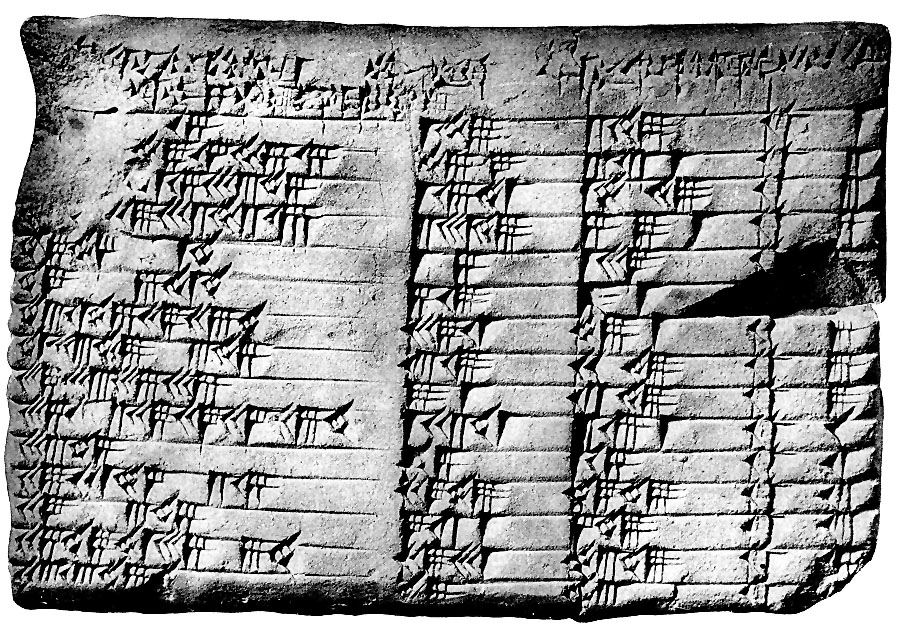
\includegraphics[width=10cm]{pic/Plimpton_322.jpg}
  \end{center}

  \caption{La tablilla babilónica Plimpton 322 (cerca de 1800 a. C.) que enumera
    algunas ternas pitagóricas. Véase \cite[\S I.V]{Weil-history}}
\end{figure}

Las ternas pitagóricas corresponden a los enteros de Gauss cuya norma es un
cuadrado: $N (x+yi) = z^2$. Puesto que $N (\alpha^2) = N (\alpha)^2$, podemos
generar las ternas pitagóricas tomando cuadrados de los enteros de Gauss.
Por ejemplo,
\[ (2 + i)^2 = 3 + 4i, \quad
   (3 + 2i)^2 = 5 + 12i, \quad
   (4 + 3i)^2 = 7 + 24i. \]

En general, tenemos $(a + bi)^2 = a^2 - b^2 + 2ab i$, así que para cualesquiera
$a,b \in \ZZ$ se obtiene una terna pitagórica
\begin{equation}
  \label{eqn:cuadrado-de-entero-de-gauss}
  (a^2 - b^2, \, 2ab, \, a^2 + b^2).
\end{equation}

Nuestro objetivo es probar que esencialmente todas las ternas pitagóricas surgen
de esta manera.

Notamos que si $(x,y,z)$ es una terna pitagórica, entonces $(cx, cy, cz)$
también lo es para cualquier $c \in \ZZ$. Por este motivo será conveniente
considerar solamente las ternas \textbf{primitivas} que satisfacen
$\gcd (x,y,z) = 1$ (lo que también equivale a $\gcd (x,y) = 1$). Las ternas
primitivas corresponden a los puntos \emph{racionales} en el círculo unitario
$x^2 + y^2 = 1$, como por ejemplo
\[ \Bigl(\frac{3}{5}, \frac{4}{5}\Bigr), ~
   \Bigl(\frac{5}{13}, \frac{12}{13}\Bigr), ~
   \Bigl(\frac{7}{25}, \frac{24}{25}\Bigr). \]

Si $(x,y,z)$ es una terna primitiva, se ve que $x$ e $y$ no pueden ser impares
al mismo tiempo. Efectivamente, en el caso contrario $x^2 + y^2 \equiv 1 + 1 = 2
\pmod{4}$, pero los cuadrados módulo $4$ son $0$ y $1$. Entonces, sin pérdida de
generalidad (intercambiando $x$ e $y$ si necesario), se puede suponer que $x$ es
impar e $y$ es par, de acuerdo con la expresión
\eqref{eqn:cuadrado-de-entero-de-gauss}.

\begin{teorema}
  Sea $(x,y,z)$ una terna pitagórica primitiva, donde $x$ es impar e $y$ es
  par. Luego, existen enteros coprimos $a > b > 0$ tales que
  $$x = a^2 - b^2, \quad y = 2ab, \quad z = a^2 + b^2.$$

  \begin{proof}
    Consideremos el entero de Gauss $x + yi$. Por nuestra hipótesis,
    $$N (x + yi) = (x + yi)\,(x - yi) = z^2.$$

    No es difícil ver que si $x$ e $y$ son coprimos y tienen diferente paridad,
    entonces $\gcd (x + yi, \, x - yi) = 1$ (ejercicio). Usando esto y el hecho
    de que su producto es un cuadrado,
    \emph{gracias a la factorización única en $\ZZ [i]$} podemos concluir que
    $x \pm yi$ son también cuadrados; existen $\alpha = a + bi \in \ZZ[i]$ y
    $u \in \ZZ[i]^\times$ tales que
    $$x+yi = u\alpha^2 = u\,(a^2 - b^2 + 2ab i).$$
    Dado que $-1 = i^2$, podemos asumir que $u \in \{ +1, +i \}$. Nuestra
    hipótesis de que $x$ es impar e $y$ es par implica que $u = +1$. Además,
    $x,y > 0$, así que $a > b > 0$. En fin, $\gcd (x,y) = 1$ implica que
    $\gcd (a,b) = 1$.
  \end{proof}
\end{teorema}

Nuestra demostración usa de manera esencial la factorización única en
$\ZZ [i]$. A saber, usamos que si $\alpha\beta = \gamma^2$ para
$\gcd (\alpha,\beta) = 1$, entonces $\alpha \sim \alpha'^2$ y
$\beta \sim \beta'^2$ para algunos $\alpha', \beta'$. Sin factorización
única no se puede llegar a esta conclusión.

\begin{ejemplo}
  Consideremos el anillo $\ZZ [\sqrt{-5}]$. En este caso las unidades son
  $\ZZ [\sqrt{-5}]^\times = \{ \pm 1 \}$. Los números
  $$\alpha = 2 + 3\sqrt{-5}, \quad \overline{\alpha} = 2 - 3\sqrt{-5}$$
  tienen norma
  $$N (\alpha) = \alpha\overline{\alpha} = 7^2.$$
  Dado que $a^2 + 5b^2 \ne 7$ para ningún $a,b \in \ZZ$,
  se ve que $\alpha$ y $\overline{\alpha}$ son irreducibles, no asociados entre
  sí. Su producto es un cuadrado, pero no son asociados con cuadrados
  (¡son irreducibles!). Aquí no hay ninguna contradicción porque
  $\ZZ [\sqrt{-5}]$ no es un dominio de factorización única.
\end{ejemplo}

%%%%%%%%%%%%%%%%%%%%%%%%%%%%%%%%%%%%%%%%%%%%%%%%%%%%%%%%%%%%%%%%%%%%%%%%%%%%%%%%

\section{Ecuación de Fermat \texorpdfstring{$x^3 + y^3 = z^3$}{$x³ + y³ = z³$}}

El lector probablemente ha escuchado del \textbf{último teorema de Fermat} que
afirma que para $n \ge 3$ la ecuación $x^n + y^n = z^n$ no tiene soluciones
enteras con $xyz \ne 0$. La prueba de este resultado (concluida por Andrew Wiles
en 1995) fue uno de los logros más publicitados de las matemáticas del siglo
pasado.

El caso particular de $n = 3$ fue resuelto por Euler. Aquí vamos a ver una
demostración con los enteros de Eisenstein $\ZZ [\zeta_3]$. Curiosamente,
el mismo Euler trabajaba con el anillo más pequeño
$\ZZ [\sqrt{-3}] \subsetneq \ZZ [\zeta_3]$, suponiendo erróneamente que este
tiene factorización única. (Véase \cite[Chapter 2]{Edwards-1996} para más
detalles.)

Antes de lanzarnos en la prueba, notamos que con las terceras raíces de la
unidad la ecuación de Fermat se factoriza como
$$x^3 + y^3 = (x + y)\,(x + \zeta_3 y)\,(x + \zeta_3^2 y) = z^3,$$
y esto explica la utilidad de los enteros de Eisenstein en nuestro problema.

\vspace{1em}

\marginpar{\small Lectura\\adicional}

Para el resto de esta sección fijemos el primo de Eisenstein
$\pi = 1 - \zeta_3$. Recordemos que $\ZZ [\zeta_3]/(\pi) \cong \FF_3$.

\begin{lema}
  \label{lema:FLT-3-1}
  La ecuación $x^3 + y^3 = uz^3$, donde $u \in \ZZ [\zeta_3]^\times$, no tiene
  soluciones $x,y,z \in \ZZ [\zeta_3]$ con $\pi \nmid xyz$.

  \begin{proof}
    Primero notamos que si $\pi \nmid x$, entonces $x \equiv \pm 1 \pmod{\pi}$,
    lo cual implica que $x^3 \equiv \pm 1 \pmod{\pi^4}$. Por ejemplo,
    si $x \equiv 1 \pmod{\pi}$, podemos escribir $x = 1 + \pi t$ para
    $t \in \ZZ [\zeta_3]$ y factorizar
    \[ x^3 - 1 = (x - 1)\,(x - \zeta_3)\,(x - \zeta_3^2)
           = \cdots = \pi^3 \, t \, (t + 1) \, (t - \zeta_3^2). \]
    Aquí $\zeta_3^2 \equiv 1 \pmod{\pi}$, y para cualquier residuo
    $t \equiv 0, +1, -1 \pmod{\pi}$ se ve que $x^3 - 1 \equiv 0 \pmod{\pi^4}$.

    Ahora bien, si $x^3 + y^3 = uz^3$ y $\pi \nmid xyz$, entonces
    $$\pm 1 \pm 1 \equiv \pm u \pmod{\pi^4}.$$
    Es fácil verificar que todas las opciones para los signos $\pm$ y
    $u \in \ZZ [\zeta_3]^\times$ nos llevan a una contradicción (note que
    $\pi^4 \sim 9$, así que se trata de los restos módulo $9$ en $\ZZ
    [\zeta_3]$).
  \end{proof}
\end{lema}

\begin{lema}
  \label{lema:FLT-3-2}
  Si $x^3 + y^3 = uz^3$ para $x,y,z \in \ZZ [\zeta_3]$ y
  $u \in \ZZ [\zeta_3]^\times$, y $\pi \nmid xy$, $\pi \mid z$, entonces
  $\pi^2 \mid z$.

  \begin{proof}
    Como en la prueba del lema anterior, se obtiene
    $$\pm 1 \pm 1 \equiv uz^3 \pmod{\pi^4}.$$
    Si $uz^3 \equiv \pm 2 \pmod{\pi^4}$, entonces $\pi \mid 2$, lo cual no es
    cierto. Por otra parte, si $uz^3 \equiv 0 \pmod{\pi^4}$, entonces
    $$3 v_\pi (z) = v_\pi (z^3) \ge 4,$$
    lo que implica $v_\pi (z) \ge 2$.
  \end{proof}
\end{lema}

La idea clave, que el mismo Fermat aplicó al caso de $n = 4$ el método del
descenso infinito, que en nuestro caso está contenido en el siguiente lema.

\begin{lema}[Descenso]
  \label{lema:FLT-3-3}
  Supongamos que $x^3 + y^3 = uz^3$, para $x,y,z\in \ZZ[\zeta_3]$ y
  $u \in \ZZ [\zeta_3]^\times$, donde $\gcd (x,y) = 1$, $\pi \nmid xy$,
  $v_\pi (z) \ge 2$. Entonces, existen $x_1, y_1, z_1 \in \ZZ [\zeta_3]$
  y $\epsilon \in \ZZ [\zeta_3]^\times$ tales que
  $$x_1^3 + y_1^3 = \epsilon z_1^3,$$
  y $\pi \nmid x_1 y_1$, $v_\pi (z_1) = v_\pi (z) - 1$.

  \begin{proof}
    Como hemos observado, la ecuación se factoriza como
    $$(x + y) \, (x + \zeta_3 y) \, (x + \zeta_3^2 y) = uz^3.$$
    Dado que por nuestra hipótesis
    $$v_\pi (uz^3) = 3 v_\pi (z) \ge 6,$$
    por lo menos uno de los tres factores debe ser divisible por
    $\pi^2$. Remplazando $y$ con $\zeta_3 y$ o $\zeta_3^2 y$, podemos asumir que
    $\pi^2 \mid (x + y)$. Ahora

    \begin{equation}
      \label{eqn:valuacion-x+zeta-y}
      v_\pi (x + \zeta_3 y) = v_\pi (x + y - (1 - \zeta_3) y)
          = \min \{ v_\pi (x+y), v_\pi (\pi y) \} = 1.
    \end{equation}
    De la misma manera,
    \begin{equation}
      \label{eqn:valuacion-x+zeta2-y}
      v_\pi (x + \zeta_3^2 y) = 1.
    \end{equation}
    Entonces,
    \begin{equation}
      \label{eqn:valuacion-x+y}
      v_\pi (x+y) = 3 v_\pi (z) - 2.
    \end{equation}

    Tenemos
    \begin{equation}
      \label{eqn:mcd-tres-factores-x3+y3}
      \gcd (x + y, x + \zeta_3 y) = \gcd (x + y, x + \zeta_3^2 y)
          = \gcd (x + \zeta_3 y, x + \zeta_3^2 y) = \pi.
    \end{equation}
    Por ejemplo, sea $\rho$ un primo tal que $\rho \not\sim \pi$ y
    $\rho \mid (x+y)$ y $\rho \mid (x + \zeta_3 y)$. Entonces,
    $\rho \mid (1 - \zeta_3) y = \pi y$ e $\rho \mid y$. Esto también implicaría
    que $\rho \mid x$, pero $\gcd (x,y) = 1$ por nuestra hipótesis. Entonces,
    el único primo que divide a $x + y$ e $x + \zeta_3 y$ es $\pi$.

    Usando \eqref{eqn:valuacion-x+zeta-y}, \eqref{eqn:valuacion-x+zeta2-y},
    \eqref{eqn:valuacion-x+y}, \eqref{eqn:mcd-tres-factores-x3+y3} podemos
    escribir
    \begin{align*}
      \tag{a} x + y & = u_1 \alpha^3 \pi^{3 v_\pi (z) - 2},\\
      \tag{b} x + \zeta_3 y & = u_2 \beta^3 \pi,\\
      \tag{c} x + \zeta_3^2 y & = u_2 \beta^3 \pi,
    \end{align*}
    donde $\pi \nmid \alpha\beta\gamma$, $u_1,u_2,u_3 \in \ZZ [\zeta_3]^\times$ y
    $$\gcd (\alpha,\beta) = \gcd (\alpha,\gamma) = \gcd (\beta,\gamma) = 1.$$

    La ecuación $\mathrm{(a)} + \zeta_3 \mathrm{(b)} + \zeta_3^2 \mathrm{(c)}$
    nos da
    \[ (\underbrace{1 + \zeta_3 + \zeta_3^2}_{=0})\,(x + y)
           = u_1 \alpha^3 \pi^{3 v_\pi (z) - 2}
                 + \zeta_3 u_2 \beta^3 \pi
                 + \zeta_3^2 u_2 \beta^3 \pi. \]
    Al cancelar $\pi$, nos queda
    \[ \zeta_3 u_2 \beta^3 + \zeta_3^2 u_2 \beta^3
           = -u_1 \alpha^3 \pi^{3 (v_\pi (z) - 1)}. \]
    Pongamos
    $$x_1 = \beta, \quad y_1 = \gamma, \quad z_1 = \alpha \pi^{v_\pi (z) - 1}.$$
    Entonces, para ciertas unidades
    $\epsilon_1, \epsilon_2 \in \ZZ[\zeta_3]^\times$ se cumple
    $$x_1^3 + \epsilon_1 y_1^3 = \epsilon_2 z_1^3.$$
    Tenemos
    $$v_\pi (z_1^3) = 3 v_\pi (z) - 3 > 2,$$
    así que la reducción módulo $\pi^2$ nos da
    $$\pm 1 \pm \epsilon_1 \equiv 0 \pmod{\pi^2}.$$
    Analizando todas las posibilidades para
    $\epsilon_1 \in \ZZ [\zeta_3]^\times$ notamos que la única posibilidad es
    $\epsilon_1 = \mp 1$. Remplazando $y$ por $-y$ si necesario, llegamos a la
    ecuación de la forma
    $$x_1^3 + y_1^3 = \epsilon z_1^3,$$
    donde $\epsilon \in \ZZ [\zeta_3]^\times$, $\pi \nmid x_1 y_1$,
    $v_\pi (z_1) = v_\pi (z) - 1$.
\end{proof}
\end{lema}

Notamos que los argumentos de arriba usan la factorización única en
$\ZZ [\zeta_3]$. Ahora estamos listos para probar el último teorema de Fermat
para $n = 3$. Ya que hemos trabajado con el anillo $\ZZ [\zeta_3]$,
el resultado será un poco más general.

\begin{teorema}
  La ecuación $x^3 + y^3 = uz^3$ para $u \in \ZZ [\zeta_3]^\times$ no tiene
  soluciones $x,y,z \in \ZZ [\zeta_3]$ con $xyz \ne 0$.

  \begin{proof}
    Asumamos que $x^3 + y^3 = uz^3$. El lema~\ref{lema:FLT-3-1} dice que
    necesariamente $\pi \mid xyz$.

    Supongamos que se cumple $\pi \nmid xy$ e $\pi \mid z$. Consideremos la
    solución con el valor de $v_\pi (z)$ más pequeño posible (entre todas las
    posibilidades para $u \in \ZZ [\zeta_3]^\times$). En este caso los
    lemas~\ref{lema:FLT-3-2} y \ref{lema:FLT-3-3} nos llevan a una
    contradicción.

    En fin, supongamos que $\pi \mid x$ y $\pi \nmid yz$. En este caso
    $u \equiv \pm 1 \pmod{\pi^3}$. Sin embargo, esto implica que $u = \pm 1$ y
    la ecuación puede ser escrita como $(\mp z)^3 + (-y)^3 = x^3$, lo cual
    corresponde al caso anterior.
  \end{proof}
\end{teorema}

\begin{comentario}
  De manera parecida, el se puede probar que $x^4 + y^4 = z^4$ no tiene
  soluciones no triviales, usando los enteros de Gauss $\ZZ [i]$. De hecho, el
  argumento demostraría el resultado para $x,y,z\in \ZZ [i]$. En este caso hay
  que considerar el primo $\pi = 1 + i$ (note que $\pi^2 \sim 2$). Para los
  detalles, véase por ejemplo \cite[\S I.3]{Ribenboim-FLT}.

  Estas pruebas usan la factorización única en los anillos ciclotómicos
  $\ZZ [\zeta_3]$ y $\ZZ [i] = \ZZ [\zeta_4]$. En general, $\ZZ [\zeta_n]$
  no tiene factorización única. Curiosamente, esto falla por primera vez para
  $n = 23$.

  Los métodos mencionados establecen algunos casos particulares del último
  teorema de Fermat para anillos de números más grandes que $\ZZ$. Sin embargo,
  el caso general de $n \ge 3$ es un problema abierto: no se sabe si la ecuación
  de Fermat $x^n + y^n = z^n$ no tiene soluciones no triviales en $\ZZ [i]$,
  $\ZZ [\zeta_3]$, etc.\footnote{Véase por ejemplo
    \url{https://mathoverflow.net/questions/90972/} y \cite{Turcas-2018}
    para el reciente progreso.}
\end{comentario}

%%%%%%%%%%%%%%%%%%%%%%%%%%%%%%%%%%%%%%%%%%%%%%%%%%%%%%%%%%%%%%%%%%%%%%%%%%%%%%%%

\section{Puntos enteros en curvas \texorpdfstring{$y^2 = x^3 + t$}{y² = x³ + t}}

Consideremos la curva plana definida por la ecuación
$$E\colon y^2 = x^3 - 1.$$

\begin{figure}
  \begin{center}
    \includegraphics{pic/y2-x3-1.pdf}
  \end{center}

  \caption{Curva elíptica $y^2 = x^3 - 1$}
  \label{fig:y2-x3-1}
\end{figure}

Un famoso teorema de Siegel nos dice que el conjunto de los puntos enteros sobre
cualquier curva elíptica
$$E\colon x^3 + ax + b, \quad a, b \in \ZZ, ~ 4a^3 + 27 b^2 \ne 0$$
es siempre finito \cite[\S X.3]{Silverman-GTM106}. En este caso particular,
una búsqueda sugiere que la única solución es $(1,0)$, pero ¿cómo probarlo?

\begin{proposicion}
  La ecuación $y^2 = x^3 - 1$ tiene única solución entera $(x,y) = (1,0)$.

  \begin{proof}
    Supongamos que $x,y\in \ZZ$ cumplen $y^2 = x^3 - 1$. Primero notamos que
    $x^3 - 1 \not\equiv 1 \pmod{4}$, así que $y$ debe ser par. En el anillo
    $\ZZ [i]$ podemos factorizar nuestra expresión como
    $$x^3 = (y+i)\,(y-i).$$
    Dejo como un ejercicio comprobar que para $y$ par se tiene
    $\gcd (y+i,y-i) = 1$. Luego, puesto que $y+i$ e $y-i$ son coprimos y su
    producto es un cubo, se cumple
    $$y + i = u\,(a + bi)^3,$$
    para algunos $u \in \ZZ [i]^\times$, $a,b \in \ZZ$. Todo elemento de
    $\ZZ [i]^\times = \{ \pm 1, \pm i \}$ es un cubo, así que sin pérdida de
    generalidad $u = 1$. Tenemos
    $$y + i = (a + bi)^3 = a\,(a^2 - 3b^2) + b\,(3a^2 - b^2)\,i.$$
    De $1 = b\,(3a^2 - b^2)$ se ve que la única solución posible es
    $a = 0, b = -1$. Esto nos permite concluir que $y = 0$, y luego $x = 1$.
  \end{proof}
\end{proposicion}

Ahora consideremos la ecuación parecida
$$y^2 = x^3 - 19.$$
Podemos tratar de aplicar el mismo truco y factorizar en
el anillo $\ZZ [\sqrt{-19}]$
$$x^3 = (y + \sqrt{-19})\,(y - \sqrt{-19}).$$

Notamos que $x^3 - 19 \not\equiv 1 \pmod{8}$, mientras que
$y^2 \equiv 1 \pmod{8}$ si $y$ es impar. Entonces, $y$ es necesariamente par,
y además se ve que $y \ne 0$. En este caso
$\gcd (y + \sqrt{-19}, y - \sqrt{-19}) = 1$, en el sentido que
$$(y + \sqrt{-19}, y - \sqrt{-19}) = \ZZ [\sqrt{-19}].$$
(¡Ejercicio!) Como antes, podemos escribir
\[ y + \sqrt{-19} = (a + b\sqrt{-19})^3
       = a\,(a^2 - 57b^2) + b\,(3a^2 - 19b^2)\,\sqrt{-19}. \]
(Note que $\ZZ [\sqrt{-19}]^\times = \{ \pm 1 \}$, así que podemos olvidar de la
unidad.) En particular, $b\,(3a^2 - 19b^2) = 1$, pero esta ecuación no tiene
soluciones enteras. Entonces, parece que la ecuación $y^2 = x^3 - 19$ no tiene
soluciones enteras\dots{} Sin embargo, no es difícil verificar que
$$7^3 - 19 = 324 = 18^2,$$
así que $(7, \pm 18)$ es una solución entera. Entonces, nuestra lógica nos
falló en algún momento.

\vspace{1em}

El problema es que el anillo $\ZZ [\sqrt{-19}]$, a diferencia de $\ZZ [i]$,
no tiene factorización única (véanse los ejercicios para una prueba).
Con las herramientas que vamos a desarrollar en nuestro curso, veremos que
el anillo más grande $\ZZ \Bigl[\frac{1+\sqrt{-19}}{2}\Bigr]$ sí tiene
factorización única, así que hay que trabajar en este anillo.

\begin{proposicion}
  Las únicas soluciones enteras de la ecuación $y^2 = x^3 - 19$ son
  $(x,y) = (7, \pm 18)$.

  \begin{proof}
    Denotemos $\alpha = \frac{1+\sqrt{-19}}{2}$. Notamos que
    $\alpha^2 - \alpha + 5 = 0$. Como mencionamos, $\ZZ [\alpha]$ tiene
    factorización única. Tenemos $\ZZ [\alpha]^\times = \{ \pm 1 \}$.
    El argumento de arriba nos da
    \[ (y-1) + 2\alpha = y + \sqrt{-19} = \left(a + b\alpha\right)^3
           = (a^3 - 15ab^2 - 5b^3) + (3a^2 + 3ab - 4b^2)\,b \alpha. \]
    La ecuación $(3a^2 + 3ab - 4b^2)\,b = 2$ implica que $b = \pm 1$, $\pm 2$,
    y se ve que las únicas soluciones enteras son
    $$(a,b) = (-2,1), (1,1).$$
    Sustituyendo estos valores, llegamos precisamente a $y = \pm 18$, y luego
    $x^3 = 18^2 + 19 = 343$, así que $x = 7$.
  \end{proof}
\end{proposicion}

\begin{figure}
  \begin{center}
    \includegraphics{pic/y2-x3-19.pdf}
  \end{center}

  \caption{Curva elíptica $y^2 = x^3 - 19$}
  \label{fig:y2-x3-19}
\end{figure}

\begin{ejemplo}
  He aquí los puntos enteros sobre algunas curvas de la forma $y^2 = x^3 + t$.
  Para la teoría detrás de esta ecuación diofántica, véase por ejemplo
  \cite{Cohen-GTM239}.

  \begin{center}
    \begin{tabular}{ll|ll}
      $y^2 = x^2 + 1\colon$ & $(-1,0), (0,\pm 1), (2,\pm 3)$ & $y^2 = x^3 - 1\colon$ & $(1,0)$ \\
      $y^2 = x^2 + 2\colon$ & $(-1,\pm 1)$ & $y^2 = x^3 - 2\colon$ & $(3,\pm 5)$ \\
      $y^2 = x^2 + 3\colon$ & $(1,\pm 2)$ & $y^2 = x^2 - 3\colon$ & --- \\
      $y^2 = x^2 + 4\colon$ & $(0,\pm 2)$ & $y^2 = x^2 - 4\colon$ & $(2,\pm 2), (5,\pm 11)$ \\
      $y^2 = x^2 + 5\colon$ & $(-1,\pm 2)$ & $y^2 = x^2 - 5\colon$ & --- \\
      $y^2 = x^2 + 6\colon$ & --- & $y^2 = x^2 - 6\colon$ & --- \\
      $y^2 = x^2 + 7\colon$ & --- & $y^2 = x^2 - 7\colon$ & $(2,\pm 1), (32,\pm 181)$ \\
      $y^2 = x^2 + 8\colon$ & $(-2,0), (1,\pm 3), (2,\pm 4), (46,\pm 312)$ & $y^2 = x^2 - 8\colon$ & $(2,0)$ \\
      $y^2 = x^2 + 9\colon$ & $(-2,\pm 1), (0,\pm 3), (3,\pm 6), (6,\pm 15), (40,\pm 253)$ & $y^2 = x^2 - 9\colon$ & --- \\
      $y^2 = x^2 + 10\colon$ & $(-1,\pm 3)$ & $y^2 = x^2 - 10\colon$ & --- \\
    \end{tabular}
  \end{center}
\end{ejemplo}

%%%%%%%%%%%%%%%%%%%%%%%%%%%%%%%%%%%%%%%%%%%%%%%%%%%%%%%%%%%%%%%%%%%%%%%%%%%%%%%%

\section{Ecuación de Pell \texorpdfstring{$x^2 - dy^2 = 1$}{x² - dy² = 1}}
\label{sec:ecuacion-de-Pell}

Sea $d > 0$ un entero libre de cuadrados. La ecuación diofántica
$$x^2 - dy^2 = 1$$
se conoce como la \textbf{ecuación de Pell}\footnote{John Pell (1611--1685),
  matemático inglés. No hay documentos que demuestren que Pell trabajó en algún
  momento de su vida en la «ecuación de Pell»; la atribución errónea del
  nombre se debe a Euler. Así que como matemático, Pell es conocido por una
  ecuación que nunca estudió.}.
Nuestro objetivo es describir las soluciones enteras.

Por ejemplo, consideremos la ecuación $x^2 - 3y^2 = 1$ (véase la figura
\ref{fig:pell-3}). Algunas soluciones evidentes son
$$(1, 0), ~ (2, 1), ~ (7, 4).$$
Podemos usar PARI/GP para encontrar más soluciones. Basta fijarnos, por ejemplo,
en los valores de $y$, y luego $x = \pm\sqrt{1 + 3y^2}$.

\begin{figure}
  \begin{center}
    \includegraphics{pic/pell-3.pdf}
  \end{center}

  \caption{Algunos puntos enteros en la curva $x^2 - 3y^2 = 1$}
  \label{fig:pell-3}
\end{figure}

\begin{shaded}
\begin{verbatim}
? pell_sol_naive (d,n) = {
  for (y=0,n,
    if (issquare (1+d*y^2),
      print ([sqrtint (1+d*y^2), y])
    )
  )
};

? pell_sol_naive (3,10^6)
[1, 0]
[2, 1]
[7, 4]
[26, 15]
[97, 56]
[362, 209]
[1351, 780]
[5042, 2911]
[18817, 10864]
[70226, 40545]
[262087, 151316]
[978122, 564719]
\end{verbatim}
\end{shaded}

Consideremos el anillo $\ZZ [\sqrt{3}]$. Este viene con la norma
$$N (x + y\sqrt{3}) = (x + y\sqrt{3})\,(x - y\sqrt{3}) = x^2 - 3y^2,$$
y el argumento que ya hemos visto arriba demuestra que
\[ \ZZ [\sqrt{3}]^\times
       = \{ \alpha \in \ZZ [\zeta_3] \mid N (\alpha) = \pm 1 \}. \]
Considerando $x^2 - 3y^2$ módulo $4$, notamos que la norma $-1$ nunca
ocurre. Entonces, las soluciones de ${x^2 - 3y^2 = 1}$ corresponden exactamente
a las unidades $u \in \ZZ [\sqrt{3}]^\times$. Por ejemplo, la solución $(2,1)$
corresponde a la unidad $u = 2 + \sqrt{3}$, y nuestra sucesión de arriba nada
más viene de las potencias $u^n$ para $n = 0,1,2,3,\ldots$ Por ejemplo,
\begin{align*}
  (2 + \sqrt{3})^2 & = 7 + 4\sqrt{3},\\
  (2 + \sqrt{3})^3 & = 26 + 15\sqrt{3}.
\end{align*}

\begin{shaded}
\begin{verbatim}
? K = nfinit(x^2-3);
? u = 2+x;
? for (n=1,10, u=nfeltmul(K,u,2+x); print(u));
[7, 4]~
[26, 15]~
[97, 56]~
[362, 209]~
[1351, 780]~
[5042, 2911]~
[18817, 10864]~
[70226, 40545]~
[262087, 151316]~
[978122, 564719]~
\end{verbatim}
\end{shaded}

En particular, notamos que $u^m \ne u^n$ para $m \ne n$, así que la ecuación
tiene un número infinito de soluciones. De hecho, en el caso contrario
$u^{m-n} = 1$, pero los elementos de $\ZZ [\sqrt{3}]$ son números reales,
y las únicas raíces de la unidad en $\RR$ son $\pm 1$.

El número $2 + \sqrt{3}$ se llama la \textbf{unidad fundamental} y surge de la
siguiente manera.

\begin{lema}
  \label{lema:unidad-fundamental-3}
  El número $2 + \sqrt{3}$ es la unidad más pequeña
  $u \in \ZZ [\sqrt{3}]^\times$ que cumple $u > 1$.

  \begin{proof}
    Supongamos que existe una unidad $u = a + b\sqrt{3}$ que cumple
    $$1 \le u \le 2 + \sqrt{3}.$$
    Luego, $u^{-1} = a - b\sqrt{3}$, y tomando los inversos se obtiene la
    desigualdad
    $$2 - \sqrt{3} \le u^{-1} \le 1.$$
    Sumando las dos desigualdades, llegamos a
    $$1 < 3 - \sqrt{3} \le u + u^{-1} \le 3 + \sqrt{3} < 5.$$
    El número $u + u^{-1} = 2a$ es par, así que hay solo dos posibilidades:
    $$u + u^{-1} = 2 \quad\text{o}\quad u + u^{-1} = 4.$$

    La primera ecuación implica que $u = 1$, mientras que la segunda implica que
    $u = 2 + \sqrt{3}$.
\end{proof}
\end{lema}

\begin{teorema}
  Toda unidad $u \in \ZZ [\sqrt{3}]^\times$ es de la forma $\pm (2 +
  \sqrt{3})^n$ para algún $n \in \ZZ$. En otras palabras, hay isomorfismo de
  grupos
  \[ \ZZ [\sqrt{3}]^\times
       \cong \langle \pm 1\rangle \times \langle 2 + \sqrt{3}\rangle
       \cong \ZZ/2\ZZ \oplus \ZZ. \]
\end{teorema}

Este es un caso muy particular del \textbf{teorema de unidades de Dirichlet} que
será uno de los resultados más importantes del curso.

\begin{proof}
  Está claro que $\pm (2 + \sqrt{3})^n$ son unidades, hay que probar que no hay
  otras. Sea $u \in \ZZ [\sqrt{3}]^\times$ una unidad. Pasando a $u^{-1}$ y
  cambiando el signo, podemos asegurarnos de que $u \ge 1$. En este caso habrá
  algún $n = 0,1,2,3,\ldots$ tal que
  $$(2 + \sqrt{3})^n \le u < (2 + \sqrt{3})^{n+1}.$$
  Luego,
  $$1 \le u\,(2 + \sqrt{3})^{-n} < 2 + \sqrt{3},$$
  y el lema de arriba implica que $u = (2 + \sqrt{3})^n$.
\end{proof}

Ahora consideremos la ecuación $x^2 - 2011 y^2 = 1$. Empleando la búsqueda tonta
para todo $y \le N$ (como por ejemplo al inicio de esta sección), no se
encuentra ninguna solución no trivial.

\begin{shaded}
\begin{verbatim}
? #
   timer = 1 (on)
? pell_sol_naive (2011,10^7)
[1, 0]
time = 5,093 ms.
? pell_sol_naive (2011,10^8)
[1, 0]
time = 50,371 ms.
\end{verbatim}
\end{shaded}

¿Será que para $d = 2011$ la ecuación de Pell ya no tiene soluciones no
triviales por alguna razón? De hecho no, $2011$ no tiene nada de especial,
solo que en este caso la unidad fundamental es

\begin{multline*}
  22903355954053525066202335319378237605968890\\
  + 510732021116138713675018566232201605320997\,\sqrt{2011}.
\end{multline*}
Ninguna búsqueda razonable puede llegar a estos números.

\begin{shaded}
  Para calcular la unidad fundamental en un campo cuadrático real, podemos hacer
  lo siguiente.
\begin{verbatim}
? quadunit(4*3)
% = 2 + w
? quadunit(4*2011)
% = 22903355954053525066202335319378237605968890
        + 510732021116138713675018566232201605320997*w
? norm (%)
% = 1
\end{verbatim}
  Hemos escrito \texttt{quadunit(4*2011)} porque $d = 2011 \equiv 2,3 \pmod{4}$,
  y el campo $\QQ (\sqrt{2011})$ tiene discriminante $4\cdot 2011$; esto será
  explicado más adelante en el curso. Además, notamos que si
  $d \equiv 1 \pmod{4}$, entonces \texttt{quadunit($d$)} devuelve la unidad
  fundamental en el anillo $\ZZ \Bigl[\frac{1+\sqrt{d}}{2}\Bigr]$.
\end{shaded}

Salvo algunos detalles, la ecuación de Pell siempre se resuelve encontrando
la unidad fundamental correspondiente. Más adelante en el curso veremos un
algoritmo para encontrarla.

\begin{ejemplo}
  He aquí una breve lista de unidades fundamentales (es decir, las unidades más
  pequeñas tales que $u > 1$) en los anillos de la forma $\ZZ [\sqrt{d}]$
  (y $\ZZ \Bigl[\frac{1+\sqrt{d}}{2}\Bigr]$ para $d \equiv 1 \pmod{4}$).

  \renewcommand{\arraystretch}{1.5}
  \begin{center}
    \begin{tabular}{rcccccccc}
      \hline
      $R\colon $ & $\ZZ [\sqrt{2}]$ & $\ZZ [\sqrt{3}]$ & $\ZZ [\sqrt{5}]$ & $\ZZ [\sqrt{6}]$ & $\ZZ [\sqrt{7}]$ & $\ZZ [\sqrt{10}]$ & $\ZZ [\sqrt{11}]$ & $\ZZ [\sqrt{13}]$ \\
      $u\colon$ & $1 + \sqrt{2}$ & $2 + \sqrt{3}$ & $2 + \sqrt{5}$ & $5 + 2\sqrt{6}$ & $8 + 3\sqrt{7}$ & $3 + \sqrt{10}$ & $10 + 3\sqrt{11}$ & $18 + 5\sqrt{13}$ \\
      $N (u)\colon$ & $-1$ & $+1$ & $-1$ & $+1$ & $-1$ & $-1$ & $+1$ & $-1$ \\
      \hline
      $R\colon $ & & & $\ZZ \Bigl[\frac{1+\sqrt{5}}{2}\Bigr]$ & & & & & $\ZZ \Bigl[\frac{1+\sqrt{13}}{2}\Bigr]$ \\
      $u\colon$ & & & $\frac{1+\sqrt{5}}{2}$ & & & & & $1 + \frac{1+\sqrt{13}}{2}$ \\
      $N (u)\colon$ & & & $-1$ & & & & & $-1$ \\
      \hline
    \end{tabular}
  \end{center}
  \renewcommand{\arraystretch}{1}

  Invito al lector a comprobar algunos casos (de la misma manera que hicimos con
  $\ZZ [\sqrt{3}]$ en \ref{lema:unidad-fundamental-3}).
\end{ejemplo}

Para que el lector no piense que los anillos cuadráticos reales $\ZZ [\sqrt{d}]$
tienen algo especial, por ejemplo, tomemos el anillo ciclotómico
$$\ZZ[\zeta_p] \cong \ZZ[x]/(\Phi_p) = \ZZ[x]/(x^{p-1} + x^{p-2} + \cdots + x + 1).$$
Allí la división con resto de polinomios nos da
$$\Phi_p = (x+1)\,(x^{p-2} + x^{p-4} + \cdots + x^3 + x) + 1,$$
lo que demuestra que
\[ (1 + \zeta_p)^{-1} =
   - (\zeta_p + \zeta_p^3 + \cdots + \zeta_p^{p-4} + \zeta_p^{p-1}), \]
así que $1 + \zeta_p \in \ZZ [\zeta_p]^\times$. En general, en el anillo
ciclotómico $\ZZ[\zeta_n]$ habrá muchas unidades, y el grupo
$\ZZ[\zeta_n]^\times$ es finitamente generado de rango $\phi(n)/2 - 1$.
Lo veremos más adelante en el curso.

\pagebreak

\phantomsection

\addcontentsline{toc}{section}{Ejercicios}
\section*{Ejercicios}

\subsection*{Campos y anillos de números}

\begin{ejercicio}[Campos cuadráticos]
  Consideremos una extensión cuadrática $K/\QQ$ (es decir, $[K : \QQ] = 2$).

  \begin{enumerate}
  \item[a)] Demuestre que $K \cong \QQ (\sqrt{d})$ para algún entero libre de
    cuadrados $d$.

  \item[b)] Demuestre que $\QQ (\sqrt{d}) \cong \QQ (\sqrt{d'})$ si y solamente
    si $d = d'$.
  \end{enumerate}

  Advertencia: esto no funciona para el grado mayor que $2$; por ejemplo,
  no todas las extensiones cúbicas son de la forma $\QQ (\sqrt[3]{d})$.
  (¿Puede encontrar algún ejemplo?)
\end{ejercicio}

\begin{ejercicio}
  El \textbf{teorema del elemento primitivo} afirma que para todo campo
  de números $K/\QQ$ existe un elemento $\alpha$ tal que $K = \QQ (\alpha)$.

  \begin{enumerate}
  \item[a)] Revise la prueba estándar en cualquier libro de texto
    \cite[Chapter V, Theorem 4.6]{Lang-Algebra} o
    \cite[Chapter I, Theorem 5.6]{Morandi-GTM167}.

  \item[b)] Encuentre $\alpha$ para
    $K = \QQ (\sqrt{2}, \sqrt{3}, \sqrt{5})$. Exprese
    $\sqrt{2}, \sqrt{3}, \sqrt{5}$ en términos de la base estándar de
    $\QQ (\alpha)$.

  \item[c*)] Use la función \texttt{rnfequation($K$,$f$)} de PARI/GP para
    obtener el polinomio mínimo de $\alpha$.
  \end{enumerate}
\end{ejercicio}

\begin{ejercicio}
  \begin{enumerate}
  \item[a)] Demuestre que los anillos $\QQ$, $\ZZ \Bigl[\frac{1}{n}\Bigr]$,
    $\ZZ_{(p)}$ no son finitamente generados como $\ZZ$-módulos.

  \item[b)] Demuestre que un grupo abeliano $p$-divisible para un primo $p$ no
    puede ser finitamente generado.
  \end{enumerate}
\end{ejercicio}

\begin{ejercicio}
  Sea $f \in \ZZ [x]$ un polinomio mónico irreducible con coeficientes enteros.

  \begin{enumerate}
    \item[a)] Demuestre que el anillo $\ZZ [x] / (f)$ es un $\ZZ$-módulo libre
      de rango $\deg f$ y el campo $\QQ [x] / (f)$ es una extensión de $\QQ$ de
      grado $\deg f$.

    \item[b)] ¿Qué sucede si $f$ no es mónico?
  \end{enumerate}
\end{ejercicio}

\subsection*{Factorización única}

\begin{ejercicio}
  Demuestre que los anillos $\ZZ [x]$ y $k [x,y]$ (donde $k$ es un campo) no son
  dominios de ideales principales. (Son dominios de factorización única, ya que
  para cualquier DFU $R$, el anillo de polinomios $R[X]$ es también un DFU.)
\end{ejercicio}

\begin{ejercicio}
  Demuestre que el anillo de polinomios con un número infinito de variables
  $$k [x_1,x_2,x_3,\ldots] = \bigcup_{n\ge 0} k [x_1,\ldots,x_n]$$
  (unión respecto a las inclusiones naturales) no es noetheriano, pero es un
  dominio de factorización única.

  Este ejemplo explica la condición a) en \ref{thm:caracterizacion-de-DFU} que
  es más débil que la condición noetheriana.
\end{ejercicio}

\begin{ejercicio}
  Demuestre que los siguientes anillos son euclidianos respecto a su norma
  habitual:
  \[ \ZZ [\sqrt{-2}], ~ \ZZ [\sqrt{2}], ~
     \ZZ [\zeta_3] = \ZZ \Bigl[\frac{1+\sqrt{-3}}{2}\Bigr], ~
     \ZZ \Bigl[\frac{1+\sqrt{-7}}{2}\Bigr], ~
     \ZZ \Bigl[\frac{1+\sqrt{-11}}{2}\Bigr]. \]
\end{ejercicio}

\begin{ejercicio}
  En este ejercicio vamos a probar que el anillo
  $R = \ZZ \Bigl[\frac{1+\sqrt{-19}}{2}\Bigr]$ no es euclidiano.

  Supongamos que $R$ es euclidiano (respecto a alguna función
  $\delta\colon R\setminus \{0\} \to \NN$). Sea $\alpha$ un elemento no nulo
  y no invertible con el mínimo posible valor de $\delta (\alpha)$
  (es decir, si $\delta (r) < \delta (\alpha)$, entonces $r = 0$ o
  $r \in R^\times$).

  \begin{enumerate}
  \item[a)] Demuestre que para cualquier $\beta \in R$ se tiene
    $\alpha \mid \beta$, o $\alpha \mid (\beta \pm 1)$.

  \item[b)] Considere qué sucede con $\beta = 2$ y
    $\beta = \frac{1+\sqrt{-19}}{2}$ para concluir que tal $\alpha$ no existe.
  \end{enumerate}

  Más adelante en el curso veremos que $\ZZ \Bigl[\frac{1+\sqrt{-19}}{2}\Bigr]$
  es un dominio de ideales principales. De la misma manera,
  $\ZZ \Bigl[\frac{1+\sqrt{-43}}{2}\Bigr]$,
  $\ZZ \Bigl[\frac{1+\sqrt{-67}}{2}\Bigr]$,
  $\ZZ \Bigl[\frac{1+\sqrt{-163}}{2}\Bigr]$
  son dominios de ideales principales, pero no son euclidianos. La moraleja de
  este ejercicio: la noción de dominio euclidiano no tiene ningún sentido
  profundo; es puramente utilitaria y se ocupa para probar que ciertos anillos
  son dominios de ideales principales. En práctica no es fácil demostrar que
  algo es un dominio euclidiano, ni que no lo es.
\end{ejercicio}

\subsection*{Enteros de Gauss $\ZZ [i]$}

\begin{ejercicio}
  Factorice el número $210$ en $\ZZ [i]$.
\end{ejercicio}

\begin{ejercicio}
  Sean $a,b$ dos enteros coprimos de diferente paridad. Demuestre que
  $\gcd (a + bi, a - bi) = 1$ en $\ZZ [i]$. En particular, si $a$ es par,
  entonces $\gcd (a + i, a - i) = 1$.
\end{ejercicio}

\begin{ejercicio}
  Calcule $\gcd (a + i, a - i)$ y $\gcd (a + 2i, a - 2i)$ en el anillo
  $\ZZ [i]$.

  \emph{Sugerencia: la respuesta depende de $a$ módulo $2$ y $4$.}
\end{ejercicio}

\begin{ejercicio}
  Ya que nuestro curso está dedicado a números algebraicos, hemos usado el
  anillo $\ZZ [i]$ para describir las ternas pitagóricas. He aquí un modo más
  geométrico de hacerlo.

  Notamos que una terna pitagórica primitiva $(x,y,z)$ corresponde a un punto
  racional $(u,v) = \left(\frac{x}{y}, \frac{y}{z}\right)$ en el circulo
  unitario. Fijemos el punto $P = (-1,0)$ y tracemos una recta que pasa por $P$
  y tiene otra intersección $Q$ con el círculo. Esta recta tendrá la ecuación
  $$\ell\colon y = tx + t$$
  para algún $t$.

  \begin{center}
    \includegraphics{pic/circle-parametrization.pdf}
  \end{center}

  La intersección de esta recta con el círculo viene dada por
  $$Q = \left(\frac{1 - t^2}{1 + t^2}, \frac{2t}{1 + t^2}\right).$$ Demuestre
  que de esta manera los puntos racionales en el círculo unitario salvo el punto
  $P$ están en biyección con $t \in \QQ$. Escribiendo $t = \frac{b}{a}$ con
  $\gcd (a,b) = 1$, recupere nuestra parametrización de las ternas pitagóricas
  primitivas.
\end{ejercicio}

\subsection*{Campos y anillos cuadráticos}

\begin{ejercicio}
  Sea $d < 0$ un entero \emph{negativo} libre de cuadrados. Usando la norma
  correspondiente\footnote{En este caso particular,
    $N_{K/\QQ} (\alpha) = \alpha\,\sigma (\alpha)$,
    donde $\Gal (K/\QQ) = \{ 1, \sigma \}$.},
  calcule los grupos de unidades

  \begin{enumerate}
  \item[a)] $\ZZ [\sqrt{d}]^\times$,
  \item[b)] $\ZZ \Bigl[\frac{1+\sqrt{d}}{2}\Bigr]^\times$ para
    $d \equiv 1 \pmod{4}$.
  \end{enumerate}
\end{ejercicio}

\begin{ejercicio}
  Sea $d \ge 3$ un entero libre de cuadrados.

  \begin{enumerate}
    \item[a)] Demuestre que en el anillo $\ZZ [\sqrt{-d}]$ el número $2$ es
      irreducible pero no es primo.

      \emph{Sugerencia: si $d$ es par, $2 \mid (\sqrt{-d})^2$ y si $d$ es impar,
      $2 \mid (1 + \sqrt{-d})\,(1 - \sqrt{-d})$.}

    \item[b)] La misma pregunta para $\ZZ [\sqrt{d}]$ si $d \equiv 1 \pmod{4}$.

      \emph{Sugerencia: $2 \mid (\sqrt{d} + 1)\,(\sqrt{d} - 1)$.}
  \end{enumerate}
\end{ejercicio}

\begin{ejercicio}
  Consideremos el ideal $I = (2, 1 + \sqrt{-3})$ en el anillo $\ZZ [\sqrt{-3}]$.

  \begin{enumerate}
  \item[a)] Demuestre que $I$ no es principal.

    \emph{Sugerencia: use la norma.}

  \item[b)] Demuestre que $I$ es principal en el anillo más grande
    $\ZZ \Bigl[\frac{1+\sqrt{-3}}{2}\Bigr]$.
  \end{enumerate}
\end{ejercicio}

\subsection*{Enteros de Eisenstein $\ZZ [\zeta_3]$}

\begin{ejercicio}
  Factorice el número $210$ en $\ZZ [\zeta_3]$.
\end{ejercicio}

\begin{ejercicio}
  Para un primo $p\equiv 1\pmod{3}$ demuestre que en la expresión
  $4p = u^2 + 27v^2$ los números $u$ y $v$ están bien definidos salvo
  signo.

  \emph{Sugerencia: revise cómo estas expresiones surgen de los enteros de
    Eisenstein $\ZZ [\zeta_3]$ y use la factorización única en $\ZZ [\zeta_3]$.}
\end{ejercicio}

\begin{ejercicio}
  Demuestre que si $\pi\in\ZZ[\zeta_3]$ es un primo de Eisenstein tal que
  $\pi\not\sim 1-\zeta_3$, entonces $1,\zeta_3,\zeta_3^2$ no son congruentes
  módulo $\pi$.
\end{ejercicio}

\begin{ejercicio}
  Sea $\pi \in \ZZ [\zeta_3]$ un primo de Eisenstein tal que
  $N (\pi) = p \equiv 1 \pmod{3}$. Demuestre que entre sus asociados
  $\pi' \sim \pi$ precisamente uno cumple $\pi' \equiv 2 \pmod{3}$.
\end{ejercicio}

\begin{ejercicio}
  Demuestre que $\legendre{\alpha}{\pi}_3 = 1$ si y solamente si $\alpha$ es un
  residuo cúbico en $\ZZ [\zeta_3]/(\pi)$ (es decir, si la congruencia
  $x^3 \equiv \alpha \pmod{\pi}$ tiene solución en $\ZZ [\zeta_3]$).
\end{ejercicio}

\begin{ejercicio}
  Verifique sin computadora si la congruencia
  $$x^3 \equiv 2 - 3\zeta_3 \pmod{23}$$
  tiene solución en $\mathbb{Z} [\zeta_3]$.

  \emph{Sugerencia: en total en $(\mathbb{Z} [\zeta_3]/(23))^\times$ habrá
    $\frac{23^2 - 1}{3} = 177$ cubos y no es una buena idea enumerarlos uno por
    uno\dots}

  En general, dado un primo racional $p \equiv 2 \pmod{3}$, ¿cuándo $2 +
  3\zeta_3$ es un cubo módulo $p$?
\end{ejercicio}

\begin{ejercicio}[\cite{Nagell-1964}]
  Demuestre que la ecuación $x^3 + y^3 = 3z^3$ no tiene soluciones
  $x,y,z \in \ZZ [\zeta_3]$ con $z\ne 0$.
\end{ejercicio}

\subsection*{Ecuación $y^2 = x^3 + t$}

\begin{ejercicio}
  Demuestre que si $a \ne 0$ es par, entonces en el anillo $\ZZ [\sqrt{-19}]$
  $$(a + \sqrt{-19}, a - \sqrt{-19}) = \ZZ [\sqrt{-19}].$$
  (Lo ocupamos en nuestro análisis de la ecuación $y^2 = x^3 - 19$.)
\end{ejercicio}

\begin{ejercicio}
  Encuentre las soluciones enteras de $y^2 = x^3 - 4$.

  \emph{Sugerencia: $y^2 + 4 = (y + 2i)\,(y - 2i)$.}
\end{ejercicio}

\subsection*{Ecuación de Pell y grupos $\ZZ [\sqrt{d}]^\times$ y $\ZZ \Bigl[\frac{\sqrt{d}}{2}\Bigr]^\times$}

\begin{ejercicio}
  Sea $d > 1$ un entero libre de cuadrados. Demuestre que si la ecuación
  $x^2 - dy^2 = -1$ tiene soluciones enteras, entonces $x^2 - dy^2 = +1$
  también tiene soluciones enteras.
\end{ejercicio}

\begin{ejercicio}
  Consideremos la ecuación $x^2 - 3y^2 = n$ para
  $$n = 2,3,4,5,6,7,8,9,10.$$
  ¿Para cuáles de estos $n$ existen soluciones enteras? Demuestre que en este
  caso hay un número infinito de ellas.
\end{ejercicio}

\begin{ejercicio}
  Demuestre que todas las soluciones de la ecuación $x^2 - 3y^2 = 1$ con
  $x,y\ge 0$ enteros vienen dadas por la recurrencia
  \begin{gather*}
    (a_0,b_0) = (1,0), \quad (a_1,b_1) = (2,1),\\
    (a_n,b_n) = 4 (a_{n-1}, b_{n-1}) - (a_{n-2}, b_{n-2}) \text{ para }n\ge 2.
  \end{gather*}
\end{ejercicio}

\begin{ejercicio}
  Describa las soluciones enteras de las ecuaciones
  $$x^2 - dy^2 = +1 \quad\text{y}\quad x^2 - dy^2 = -1,$$
  donde $d = 2$ y $5$.
\end{ejercicio}

\begin{ejercicio}
  Consideremos el anillo $\ZZ \Bigl[\frac{1+\sqrt{5}}{2}\Bigr]$.

  \begin{enumerate}
  \item[a)] Encuentre la unidad más pequeña
    $u \in \ZZ \Bigl[\frac{1+\sqrt{5}}{2}\Bigr]^\times$ tal que $u > 1$.

  \item[b)] Encuentre el índice de subgrupo
    $\Bigl[\ZZ \Bigl[\frac{1+\sqrt{5}}{2}\Bigr]^\times :
           \ZZ [\sqrt{5}]^\times\Bigr]$.
  \end{enumerate}
\end{ejercicio}

\begin{ejercicio}
  Consideremos el anillo ciclotómico $\ZZ [\zeta_5]$.

  \begin{enumerate}
  \item[a)] Demuestre que $u = 1 + \zeta_5$ es una unidad en el anillo 
    y el subgrupo de $\ZZ [\zeta_5]^\times$ generado por $u$ es infinito.

    En realidad,
    $\ZZ [\zeta_5]^\times \cong \mu_{10} (\CC) \times \langle u\rangle$,
    pero lo probaremos más adelante en el curso.

  \item[b)] Demuestre que
    $\ZZ \Bigl[\frac{1 + \sqrt{5}}{2}\Bigr] \subset \ZZ [\zeta_5]$ y calcule
    el índice
    $\Bigl[\ZZ [\zeta_5]^\times :
           \ZZ \Bigl[\frac{1 + \sqrt{5}}{2}\Bigr]^\times \Bigr]$.
  \end{enumerate}
\end{ejercicio}
